\section{Diseño y Funcionamiento}

Como se dijo en la introducción de este capítulo, resulta natural ejecutar
una RdP dentro de un monitor de concurrencia. Así queda en evidencia la
necesidad de contar con un software capaz de ejecutar una RdP y que cumpla con
los requerimientos de un monitor de concurrencia para la realización de este
proyecto integrador.
En primera instancia se analizó la reutilización y expansión de las
funcionalidades del monitor construido en el desarrollo de \cite{codegen}, y
reutilizado en \cite{chimp}. Durante este análisis se vio que, si bien este
software cumple con los requerimientos mínimos necesarios, para agregar las
funcionalidades requeridas por este proyecto integrador era necesaria la
refactorización de la mayor parte del mismo. Además, el estilo seguido durante
su desarrollo no se condice con el estándar de Java, siendo esta otra razón
para decidir hacer una re-implementación completa del monitor.
Por esto es que, como parte del desarrollo de este proyecto integrador, se
diseñó y construyó Java Petri Concurrency Monitor (JPCM).

\subsection{Arquitectura de Alto Nivel}
\label{JPCM_arq_alto_nivel}

Según las clasificaciones vistas en las secciones
\ref{monitor_sincronizacion_explicita} y \ref{politica_monitor}, JPCM es un
monitor de sincronización explícita y aplica una política de desbloqueo de hilos
de retorno forzado.
 
Las principales partes que componen a JPCM son:
\begin{itemize}
  \item \underline{PetriNet:} contiene la información de la RdP a utilizar y la
  lógica de la ejecución
  \item \unverline{PnmlParser + PetriNetFactory:} su responsabilidad es
  convertir la información del archivo que describe a la RdP en un formato
  ejecutable para JPCM.
  \item \underline{PetriMonitor:} es el monitor en sí mismo. Expone las
  interfaces de programación y tiene la responsabilidad de gestionar los hilos
  para evitar la ejecución concurrente de la RdP.
  \item \underline{TransitionsPolicy:} representa la política de gestión de los
  recursos del monitor. No es la misma política analizada en la sección
  \ref{politica_monitor}. Esta política permite decidir cuál transición, de un
  conjunto dado, es la próxima a ser disparada.
\end{itemize}

La figura \ref{fig:JPCM_Arquitectura} es un diagrama de arquitectura de JPCM,
mostrando sus principales bloques e interacciones.

\begin{figure}[H]
  \centering
  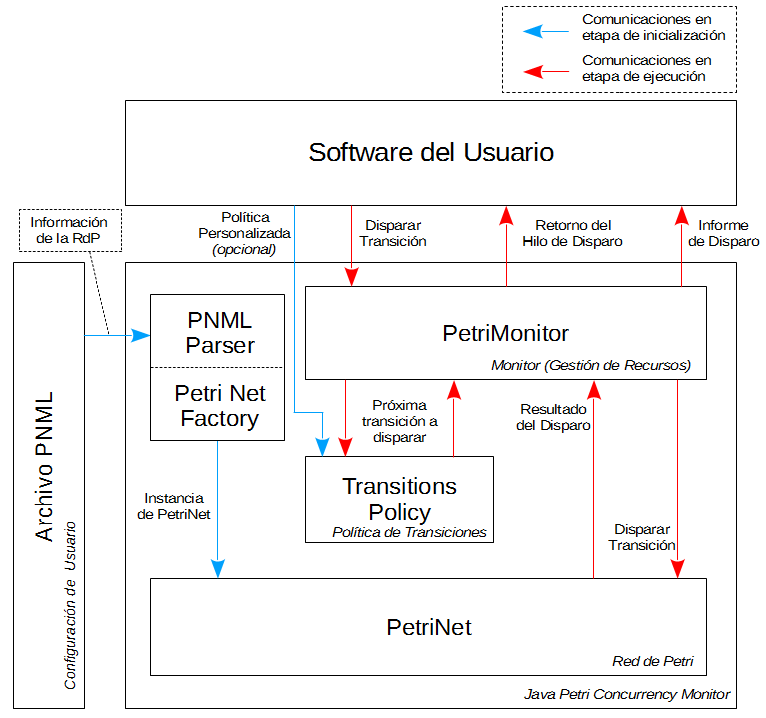
\includegraphics[width=125mm]{JPCM_Arquitectura}
  \caption{Arquitectura de JPCM}
  \label{fig:JPCM_Arquitectura}
\end{figure}

\subsection{Gestión de los Recursos con RdP}
\label{JPCM_gestion_rec_rdp}
En la sección \ref{monitores} se analiza cómo se gestionan los recursos de un
monitor con variables de condición en un monitor de sincronización explícita.
Allí se explicó cómo un hilo que desea tomar o devolver un recurso debe
señalizar a una variable de condición, y bloquearse en caso de no tener el
recurso disponible.

Por otro lado, en la sección \ref{POPN} se explica cómo una RdP puede
representar procesos. De esta manera, un hilo que quiera ejecutar el proceso
\textit{A}, debe señalizar el comienzo y fin de la ejecución en la RdP
disparando un subconjunto de transiciones de inicio y otro subconjunto de
transiciones de finalización.
 
Si bien no existe una relación directa entre las operaciones de una variable de
condición y los disparos de una transición, se logra obtener los mismos
comportamientos sobre los hilos que las acceden con la ayuda de colas
auxiliares. Esto permite establecer una semejanza entre las variables de
condición de un monitor y las transiciones de una RdP.

Cuando se intenta disparar una transición no sensibilizada, el hilo que intentó
hacer el disparo se bloquea en una cola de la misma forma que si hubiera hecho
una llamada a \textit{wait()} sobre una variable de condición. De la misma
manera, un hilo que dispara una transición $t_{0}$ y sensibiliza a otra $t_{1}$,
desbloquea a algún hilo que esperaba por $t_{1}$ como si hubiera hecho una
llamada a \textit{signal()} sobre una variable de condición.

A partir de esta semejanza queda en evidencia que las operaciones a realizar
dentro de un monitor que ejecuta una RdP consisten en el disparo de una o más
transiciones para cambiar el estado en que se encuentran los recursos y las
operaciones modeladas por ella.

\subsection{Estructura Interna de JPCM}
Basándose en el diagrama de la figura \ref{fig:JPCM_Arquitectura}, se puede
dividir a JPCM en dos secciones:
\begin{itemize}
    \item Modelo: Tiene como eje central a la clase \textit{PetriNet}. Dentro de
    esta sección se genera el modelo ejecutable con todos sus componentes. Se ayuda
    de clases auxiliares para hacer la generación del modelo
    \item Ejecución: Tiene como eje central a la clase \textit{PetriMonitor}. Se
    encarga de tomar el modelo y ejecutarlo. Incluye clases auxiliares para
    implementar las políticas del monitor (de transiciones y de colas)
\end{itemize}

\subsubsection{La Sección Modelo}
En el siguiente diagrama de clases se observan las clases que componen a esta
sección, junto con sus composiciones e interacciones estructurales:

\begin{figure}[H]
  \hspace*{-3cm}
  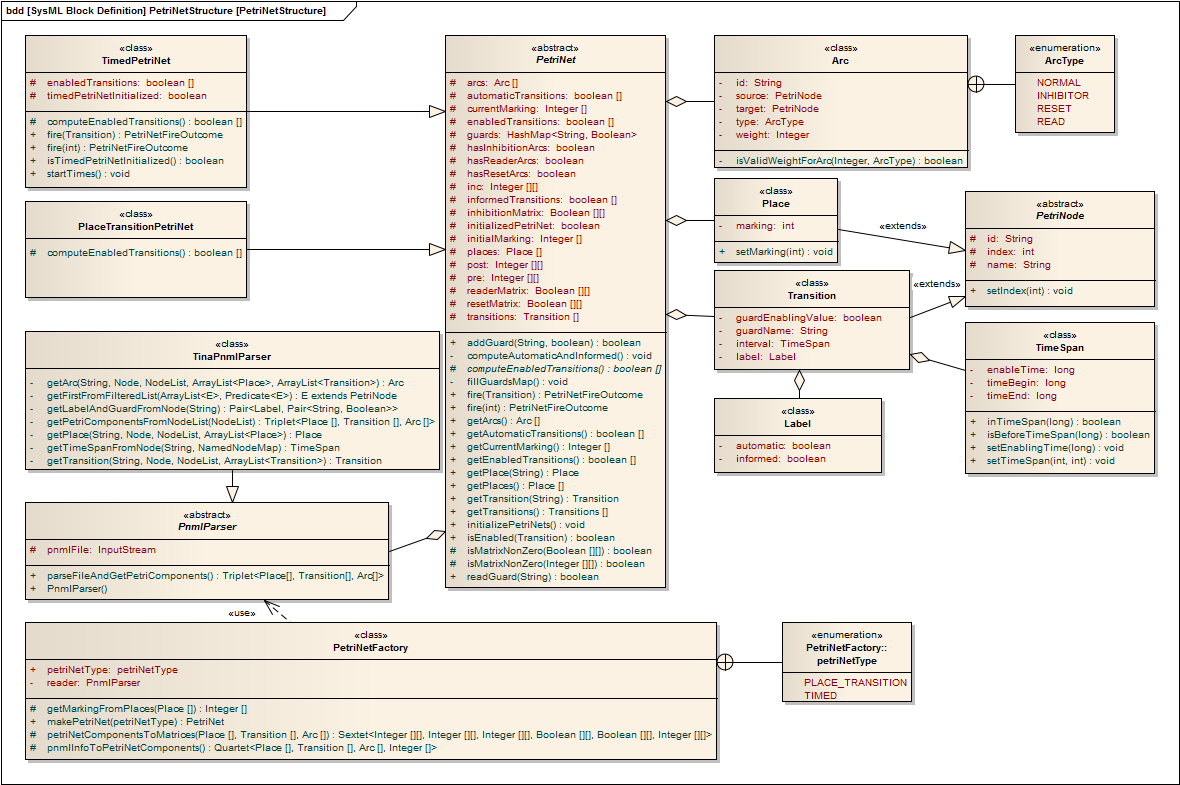
\includegraphics[width=190mm]{JPCM_PetriNet_Structure}
  \caption{Diagrama de clases de la sección \textit{Modelo}}
  \label{fig:JPCM_PetriNet_Structure}
\end{figure}

Se pueden ver las clases que modelan a los componentes de una RdP estructural
(ver sección \ref{def_formal_petri}) (\textit{Arc}, \textit{Transition},
\textit{Place}), la especializaciones concretas de \textit{PetriNet}
(\textit{PlaceTransitionPetriNet} y \textit{TimedPetriNet}), las clases
\textit{PetriNetFactory} y \textit{PnmlParser} vistas en la sección
\ref{JPCM_arq_alto_nivel} y la especialización de \textit{PnmlParser} que
comprende el dialecto PNML de TINA, \textit{TinaPnmlParser}.

\subsubsection{La sección Ejecución}
En el siguiente diagrama de clases se observan las clases que componen a la
sección Ejecución, junto con sus composiciones y relaciones estructurales:

\begin{figure}[H]
  \hspace*{-2.5cm}
  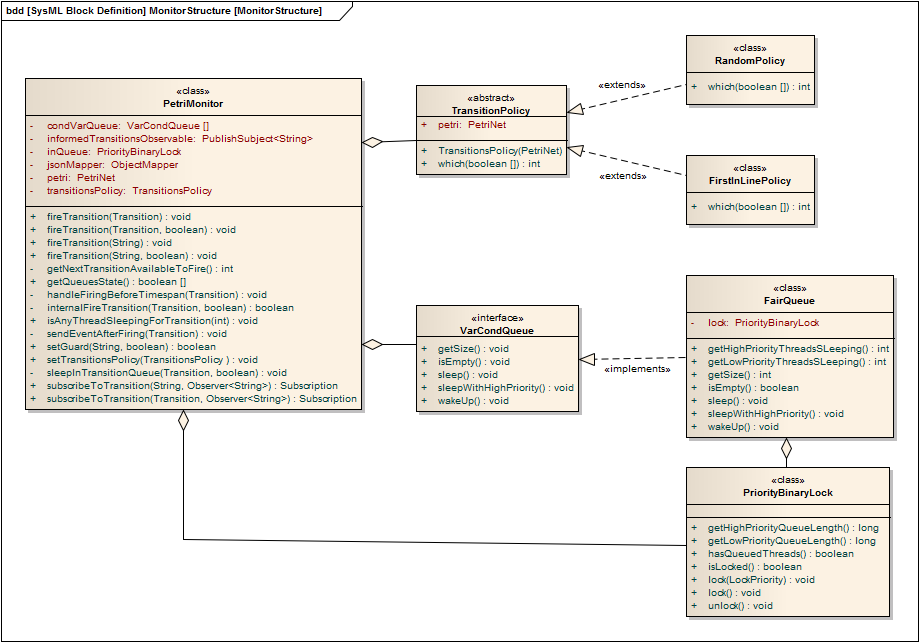
\includegraphics[width=180mm]{JPCM_PetriMonitor_Structure}
  \caption{Diagrama de clases de la sección \textit{Ejecución}}
  \label{fig:JPCM_PetriMonitor_Structure}
\end{figure}

Junto a la clase \textit{PetriMonitor} se puede ver por un lado la subsección
que aplica la política de transiciones. Por ese lado está la clase abstracta
\textit{TransitionsPolicy} y sus especializaciones \textit{RandomPolicy}
(política aleatoria) y \textit{FirstInLinePolicy} (política de primer transición
en la lista).

Por otro lado, la clase \textit{PriorityBinaryLock} (ver sección
\ref{JPCM_solucion_inv_prioridad}) implementa la política de colas por
prioridad.

Las colas de condición asociadas a las transiciones (ver sección
\ref{JPCM_gestion_rec_rdp}) están descriptas en la interfaz
\textit{VarCondQueue} e implementadas en la clase \textit{FairQueue}.


\subsection{Interfaces de Programación}

JPCM ofrece una interfaz de entrada al monitor y dos de salida en tiempo de
ejecución, y dos interfaces de carga de datos de configuración en tiempo de
inicialización.

En tiempo de ejecución, la interfaz de entrada es el método público 
\mint{java}|PetriMonitor.fireTransition()|. Este método permite disparar una
transición de la RdP dentro del monitor de concurrencia, ya sea utilizando el
objeto \textit{Transition} (transición) de la RdP, o el nombre de la misma.

Las interfaces salida son dos:
\begin{itemize}
  \item \underline{Retorno del disparo de una transición:} la finalización de
  ejecución del método \mint{java}|PetriMonitor.fireTransition()| asegura que el
  hilo que hizo la llamada, efectivamente disparó de la transición deseada
  (excepto en disparos no-perennes donde no se da esta garantía, ver sección
  \ref{disparos_perennes})
  \item \underline{Informes de disparo:} ante el disparo de una
  transición informada, se emite un evento con información sobre la transición
  disparada. Todos los observadores suscritos a estos eventos lo reciben.
\end{itemize}

En tiempo de inicialización se proveen dos interfaces al usuario:
\begin{itemize} 
  \item \underline{Carga de una RdP:} Se hace mediante un archivo descriptor
  en formato PNML. El bloque \textit{PnmlParser + PetriNetFactory} lo utiliza
  para generar una RdP ejecutable.
  \item \underline{Carga de una política personalizada:} Es opcional. Permite
  al usuario definir una política de transiciones que se ajuste al problema a
  resolver por su software.
\end{itemize}

Estas interfaces proveen al usuario de los mecanismos necesarios para
inicializar el monitor, y para luego utilizarlo para la sincronización de hilos
concurrentes.

\subsection{Inicialización de JPCM}
Antes de poder utilizar JPCM para sincronizar la ejecución de hilos con una
RdP, es necesario inicializarlo de forma correcta. Los pasos para inicializar
JPCM son:
\begin{itemize}
  \item Instanciar la clase \textit{PnmlParser} pasándole la ruta al archivo de
  descripción de la RdP a utilizar
  \item Instanciar la clase \textit{PetriNetFactory} con el objeto
  \textit{PnmlParser}
  \item Utilizar el objeto \textit{PetriNetFactory} para generar una instancia
  de \textit{PetriNet}
  \tem Instanciar una política (clases \textit{FirstInLinePolicy} o
  \textit{RandomPolicy} o alguna generada por el usuario)
  \item Instanciar la clase \textit{PetriMonitor} con el objeto
  \textit{PetriNet} y el objeto de la política
  \item Crear los hilos que van a ejecutar las tareas del sistema y asignarle
  sus tareas
  \item Inicializar la RdP llamando a \mint{java}|PetriNet.initializePetriNet()|
  sobre la instancia de \textit{PetriNet}
  \item Lanzar los hilos creados anteriormente
  \item Evitar que el hilo principal termine antes que los hilos trabajadores
\end{itemize}
 
Luego de realizar todas estas tareas, el sistema comienza a ejecutarse por sí
solo, orquestado por la RdP.

\subsubsection{Generación de una RdP Ejecutable a Partir de un Archivo PNML}
Como se dijo anteriormente, JPCM requiere de un archivo PNML con la descripción
de la RdP a utilizar. Los pasos a seguir para obtener una RdP ejecutable a
partir del archivo PNML son los siguientes:
\begin{itemize}
  \item Una instancia de PnmlParser analiza el archivo para obtener los
  componentes de RdP contenidos en él (Plazas, Arcos y Transiciones)
  \item Con la información obtenida genera objetos de tipo \textit{Place},
  \textit{Transition} o \textit{Arc} dependiendo del caso
  \item Ordena los objetos generados en tres arrays, uno por cada tipo de
  componente y los empaqueta en una tupla
  \item Cuando se llama a \mint{java}|PetriNetFactory.makePetriNet()| sobre la
  instancia de \textit{PetriNetFactory}, ésta obtiene la tupla de arrays de
  componentes generada por \textit{PnmlParser}
  \item Con los objetos componentes de la RdP, \textit{PetriNetFactory} calcula
  y almacena las matrices de precedencia, pos-incidencia, incidencia, inhibición,
  reset y lectura
  \item Con los objetos componentes, las matrices de la RdP y el tipo de RdP a
  generar, crea una instancia de la subclase de \textit{PetriNet}
  correspondiente
\end{itemize}

El objeto resultante es una RdP ejecutable que se puede utilizar en conjunto
con el monitor.

\subsection{Disparo de una Transición en JPCM}
El disparo de una transición en el monitor mediante la ejecución del método
\mint{java}|PetriMonitor.fireTransition(t)| desencadena las siguientes acciones
sobre el hilo que realiza la llamada:

\begin{itemize}
  \item \underline{Verifica que la transición t no sea automática:} En cuyo caso
  falla con un error explicando la situación
  \item \underline{Verifica que la red esté inicializada:} Si no lo está falla
  con un error explicando la situación
  \item \underline{Toma el lock sobre la entrada del monitor:} Si no lo puede
  tomar se bloquea en la cola de entrada hasta poder tomarlo
  \item \underline{Dispara la transición en la RdP:} Devuelve un código de error
  indicando el resultado
  \item \underline{Maneja el resultado del disparo:} se analiza si se debe
  liberar el lock de entrada, disparar una transición automática, liberar un
  hilo bloqueado o bloquearse por una condición
  \item \underline{Libera el lock de entrada:} Si la acción anterior determinó
  que se lo debe liberar
\end{itemize}
 
La figura \ref{fig:JPCM_Fire_General} es un diagrama de secuencias donde se
observa el flujo de un hilo que realiza un disparo de una transición:

\begin{figure}[H]
  \hspace*{-3cm}
  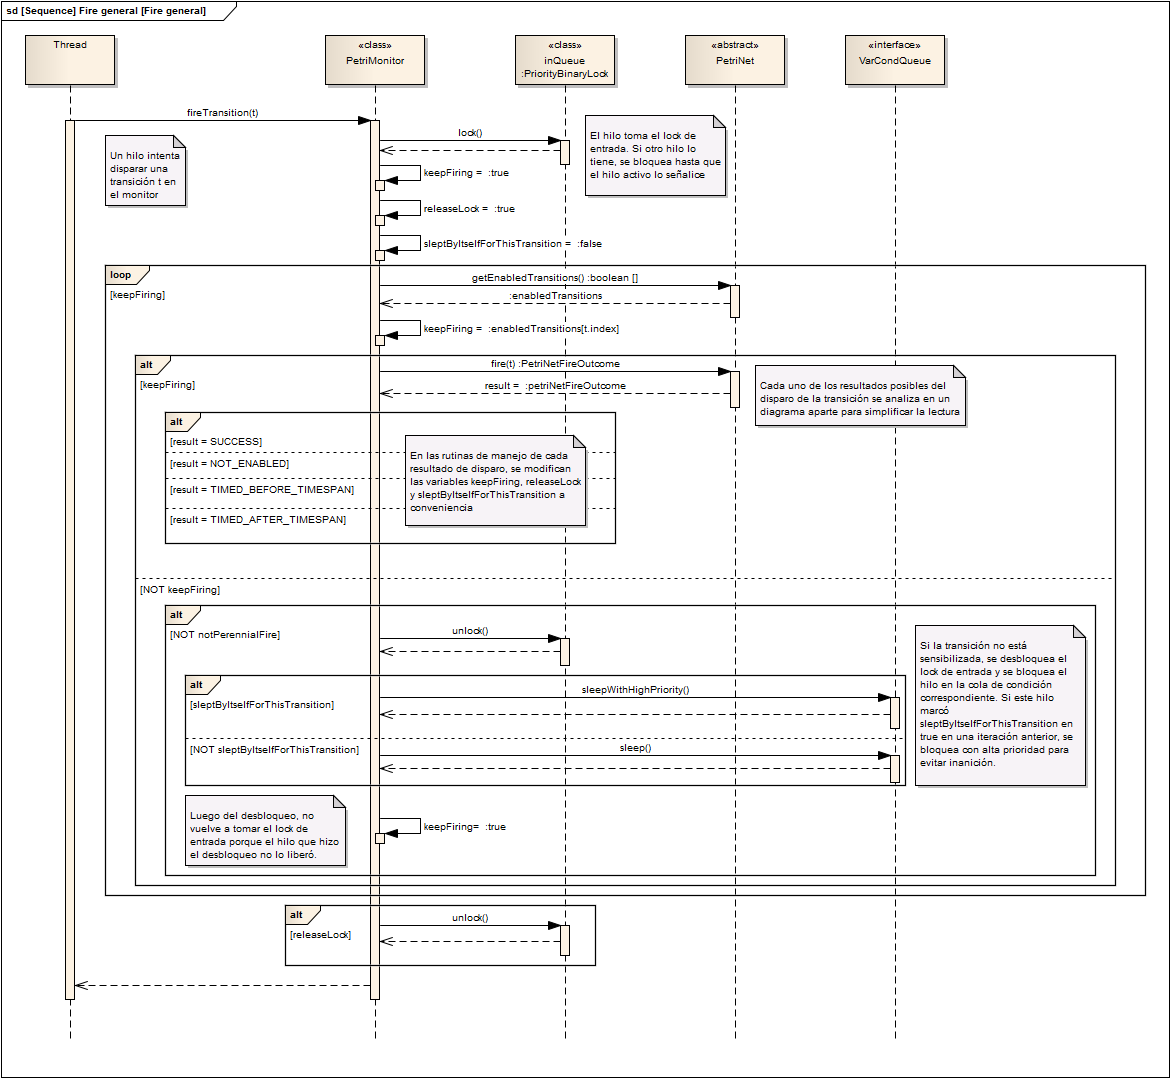
\includegraphics[width=190mm]{JPCM_Fire_General}
  \caption{Disparo de una transición}
  \label{fig:JPCM_Fire_General}
\end{figure}

\subsection*{Manejo del código de error del disparo}

Cuando se realiza el disparo efectivo de la transición en la red de petri, ésta
devuelve un código de error basado en el resultado del disparo. Estos pueden
ser:
\begin{itemize}
  \item \textit{SUCCESS:} el disparo fue exitoso
  \item \textit{NOT\_ENABLED:} la transición no está sensbilizada
  \item \textit{TIMED\_BEFORE\_TIMESTAMP:} Sólo para transiciones
  temporales. El instante de disparo es anterior al \textit{instante menor de disparo} de la transición
  (ver sección \ref{semantica_tiempo_debil})
  \item \textit{TIMED\_AFTER\_TIMESTAMP:} Sólo para transiciones
  temporales. El instante de disparo es posterior al \textit{instante mayor de disparo} de la transición
  (ver sección \ref{semantica_tiempo_debil})
\end{itemize}

\subsubsection*{Caso del disparo exitoso}
Ante un disparo exitoso, la llamada a \mint{java}|PetriNet.fire(Transition t)|
devuelve un código \textit{SUCCESS}. Una vez que esto ocurre, el hilo que
realizó el disparo debe:
\begin{itemize}
  \item Emitir un evento para todos los suscriptores (en el caso que la
  transición sea informada).
  \item Revisar si existen nuevas transiciones sensibilizadas producto del
  último disparo
  \begin{itemize}
    \item Si no existen, libera el lock de entrada y abandona el monitor
    \item Si existen:
    \begin{itemize}
        \item Consulta a la política de transiciones cuál debe ser la próxima a ser disparada
        \item De ser automática el disparo lo hace el mismo hilo, por lo que
        itera para realizar un nuevo disparo sobre la transición automática.
        \item De ser disparada debe señalizar al hilo que esté esperando en su
        cola de condición y abandonar el monitor inmediatamente sin liberar el
        lock de entrada.
    \end{itemize}
  \end{itemize}
\end{itemize}

En el siguiente diagrama de secuencias se observa en detalle el flujo de un
disparo exitoso de una transición:

\begin{figure}[H]
  \centering
  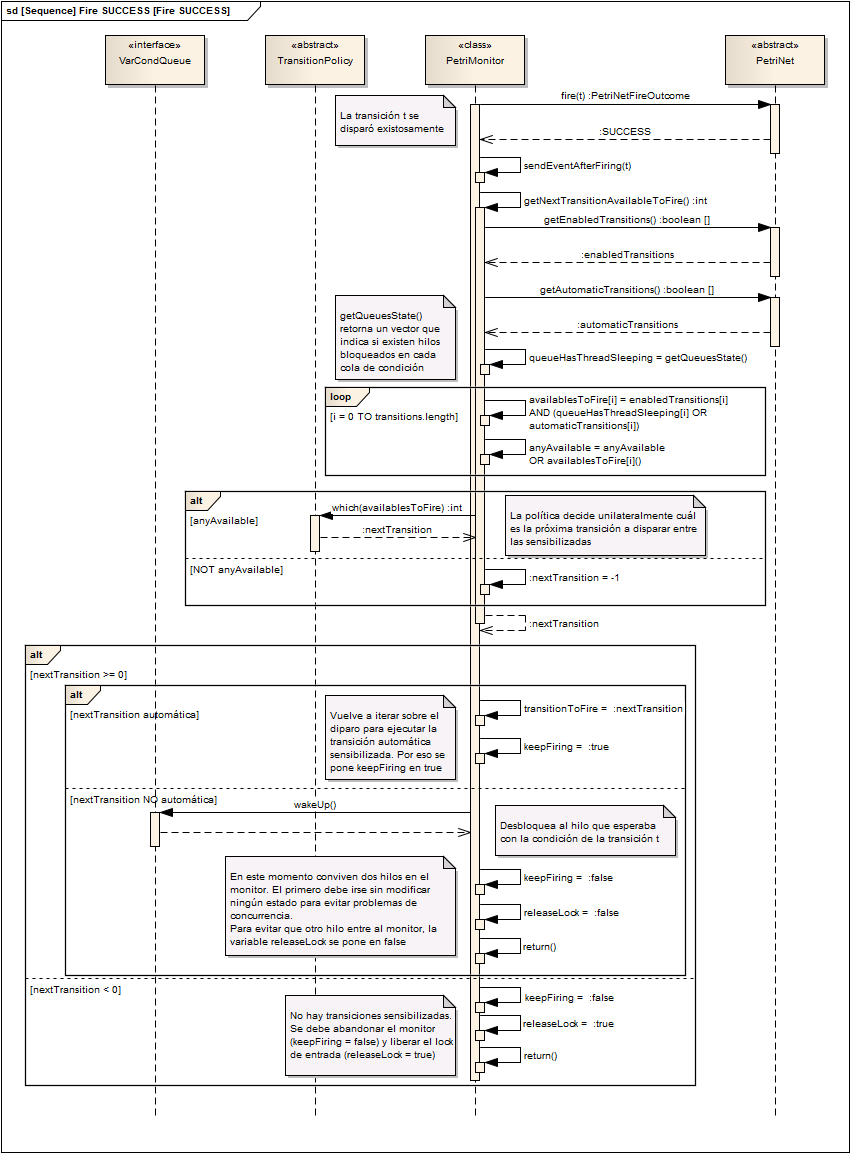
\includegraphics[width=140mm]{JPCM_Fire_SUCCESS}
  \caption{Manejo del disparo exitoso de una transición}
  \label{fig:JPCM_Fire_SUCCESS}
\end{figure}

\subsubsection*{Caso del disparo no exitoso, y del temporal después del
intervalo}

Cuando la transición no está sensibilizada, su disparo devuelve
\textit{NOT\_ENABLED}. Ante este caso, un hilo que realizó un disparo perenne
debe esperar en la cola de condición asociada a la transición. A su vez, si en
una iteración anterior realizó una espera temporal por la transición, debe
bloquearse con alta prioridad.
Ante el caso del disparo de una transición temporal en un instante posterior al
instante mayor de disparo, el resultado es \textit{TIMED\_AFTER\_TIMESPAN} y el
procedimiento a realizar es idéntico al caso anterior.
 
En el siguiente diagrama de secuencias se muestra detallado el caso del disparo
no exitoso:

\begin{figure}[H]
  \hspace*{-2cm}
  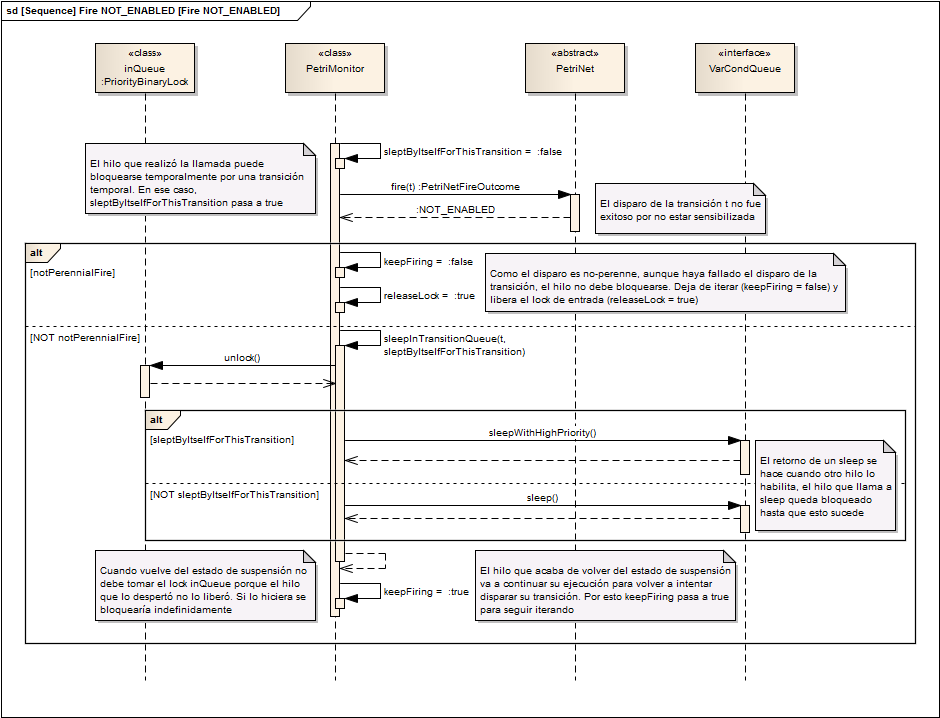
\includegraphics[width=170mm]{JPCM_Fire_NOT_ENABLED}
  \caption{Manejo del disparo no exitoso de una transición}
  \label{fig:JPCM_Fire_NOT_ENABLED}
\end{figure}

\subsubsection*{Caso del disparo temporal antes del intervalo}
Si un hilo intenta disparar una transición temporal antes del instante menor de
disparo, la llamada a \mint{java}|PetriNet.fire(Transition t)| devuelve un error
\textit{TIMED\_BEFORE\_TIMESPAN}.
En este caso, el procedimiento a seguir es el siguiente:
\begin{itemize}
  \item Si no hay hilo bloqueado por t:
  \begin{itemize}
    \item Liberar el lock de entrada
    \item Esperar temporalmente hasta el \textit{instante menor de disparo}
    \item Tomar el lock de entrada con alta prioridad {\color{red}(ver
    inversión de prioridades)}
    \item Señalizar que ya se suspendió temporalmente para evitar futuras
    inversiones de prioridad
    \item Iterar sobre el disparo para reintentarlo
  \end{itemize}
  \item Si existe un hilo bloqueado por t:
  \begin{itemize}
    \item Si el disparo es no-perenne
    \begin{itemize}
      \item Liberar el lock de entrada
      \item Abandonar el monitor
    \end{itemize}
    \item Si el disparo es perenne
    \begin{itemize}
      \item Liberar el lock de entrada
      \item Bloquearse en la cola de condición de t. Si ya se suspendió
      temporalmente por t antes, lo hace con alta prioridad {\color{red}(ver
      inversión de prioridades)}
      \item Cuando se desbloquea itera para reintentar el disparo
    \end{itemize}
  \end{itemize}
\end{itemize}
En el siguiente diagrama de secuencias se detalla el flujo de este caso de resultado de disparo.

\begin{figure}[H]
  \centering
  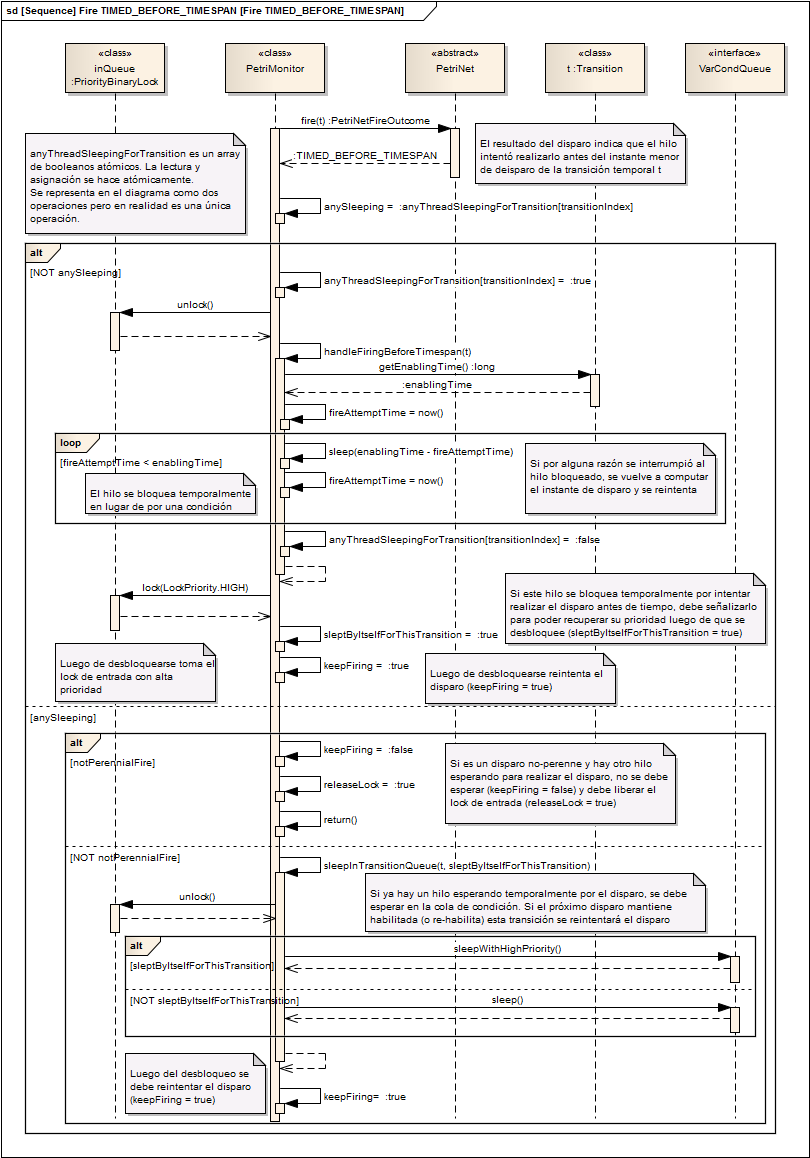
\includegraphics[width=140mm]{JPCM_Fire_TIMED_BEFORE_TIMESPAN}
  \caption{Manejo del disparo de una transición temporal antes del instante
  menor de disparo}
  \label{fig:JPCM_Fire_TIMED_BEFORE_TIMESPAN}
\end{figure}

\subsection{Problema de la Inversión de Prioridades}

Durante el desarrollo de JPCM se detectaron dos casos donde se produce una
inversión de prioridades entre los hilos gestionados. A continuación se
analizan estos casos.

\subsubsection{Inversión de prioridades en la cola de entrada}
\label{inversion_prioridad_cola_entrada}
Para lograr la inversión de prioridades en la cola de entrada se tienen que dar
los siguientes eventos en orden:
\begin{itemize}
  \item Se sensibiliza la transición temporal $t_{0}$ con intervalo $[a,b]$ en
  el instante $t_{i}$
  \item El hilo $th_{0}$ intenta disparar $t_{0}$ en $t_{d} < (t_{i} + a)$
  \item El hilo $th_{0}$ libera la entrada y se bloquea temporalmente
  \item Entra otro hilo a realizar un disparo y bloquea la entrada
  \item Llegan al monitor $N$ hilos a intentar realizar disparos y se encolan a
  la entrada
  \item Cuando $th_{0}$ se desbloquea, intenta tomar el lock de entrada y va al
  final de la cola
\end{itemize}

En este caso, $th_{0}$ cedió su prioridad a los $N$ hilos que llegaron después
que él. Esto puede resultar en que el intervalo de disparo termine antes de que
$th_{0}$ recupere su turno dentro del monitor, provocando su inanición.

En la figura \ref{fig:Inv_prior_entrada} se observa gráficamente la secuencia de
pasos para lograr la inversión de prioridades en la cola de entrada del monitor.

\begin{figure}[H]
  \centering
    \subfigure[El hilo $th_{0}$ ingresa al monitor]
    {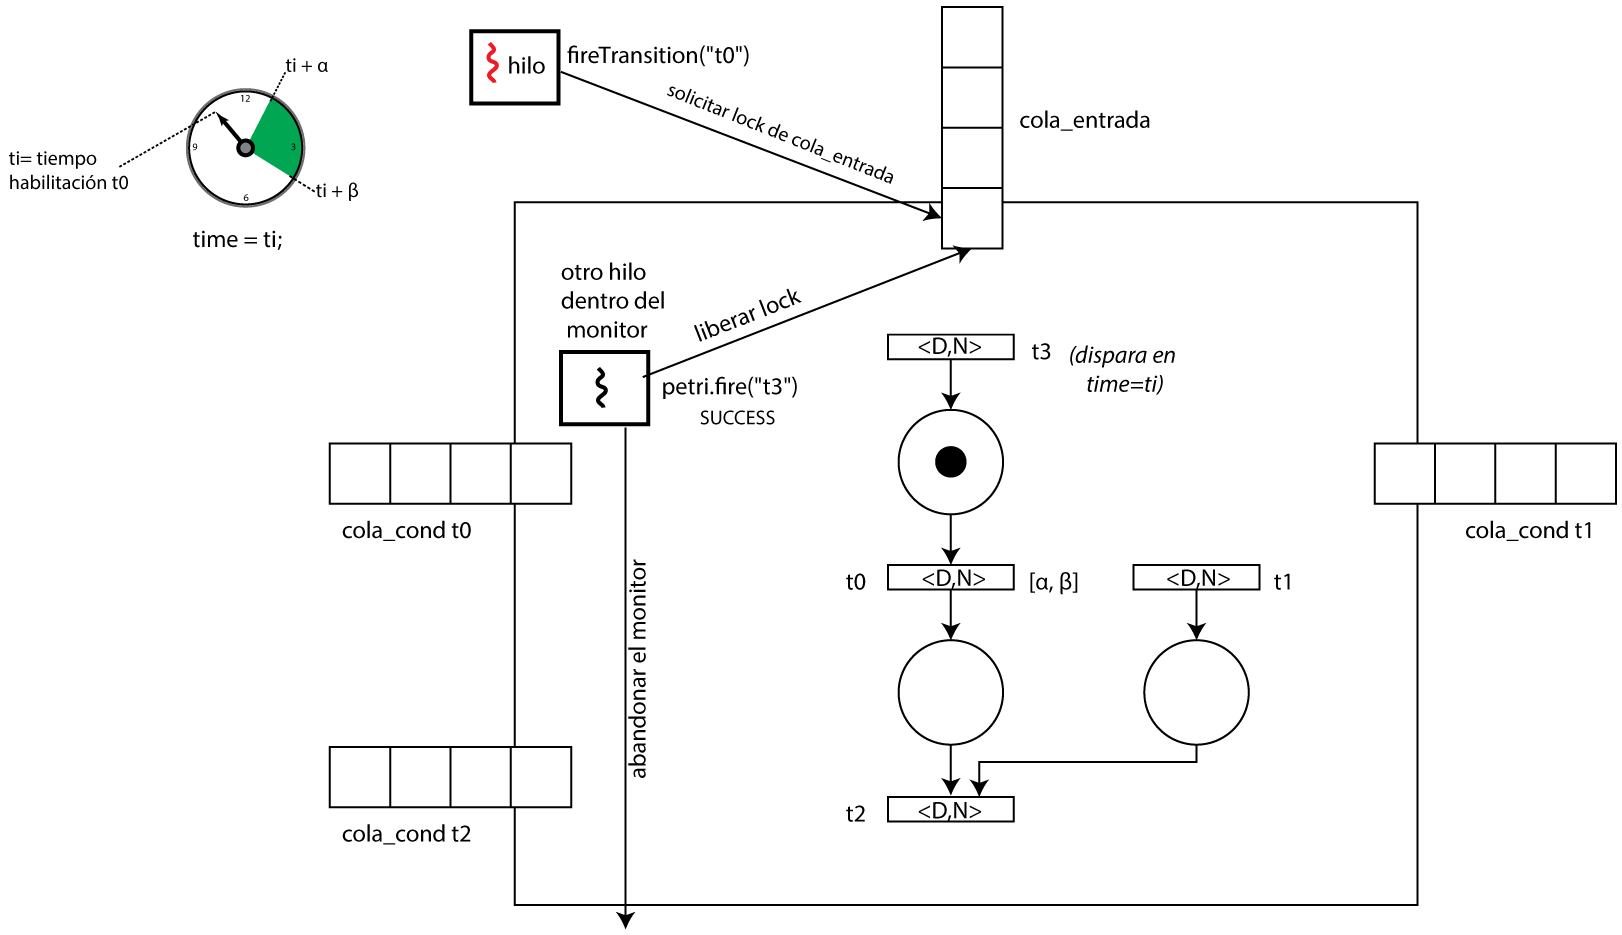
\includegraphics[width=\textwidth]{InversionPrioridad/Inversion_Prioridad_01}}
    \subfigure[El hilo $th_{0}$ intenta disparar $t_{0}$ en $t_{d} < (t_{i} + a)$]
    {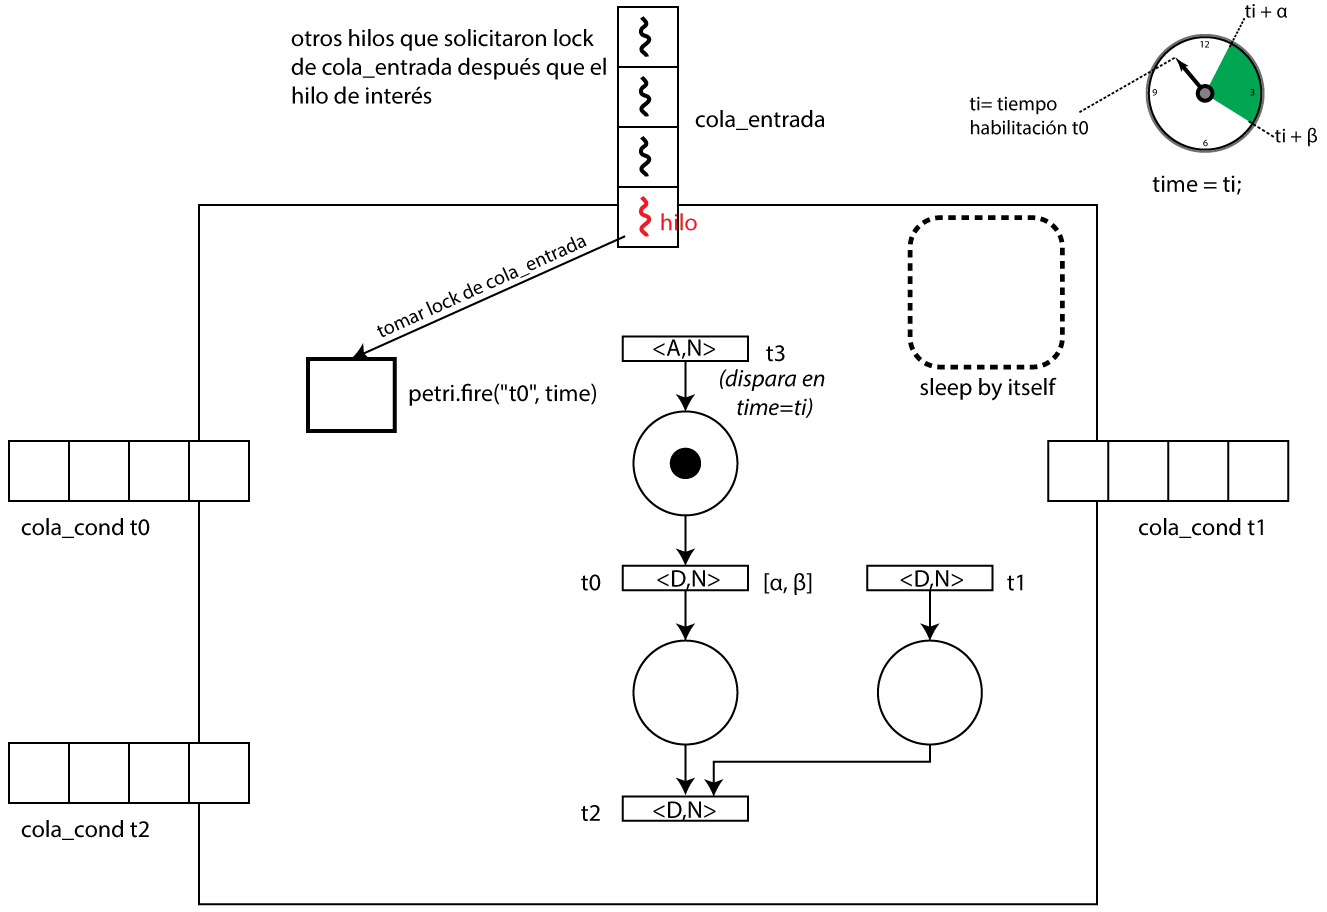
\includegraphics[width=\textwidth]{InversionPrioridad/Inversion_Prioridad_02}}
    \label{fig:Inv_prior_entrada}
    \phantomcaption
\end{figure}
\clearpage
\begin{figure}[H]
    \ContinuedFloat
    \subfigure[El hilo $th_{0}$ se bloquea temporalmente]
    {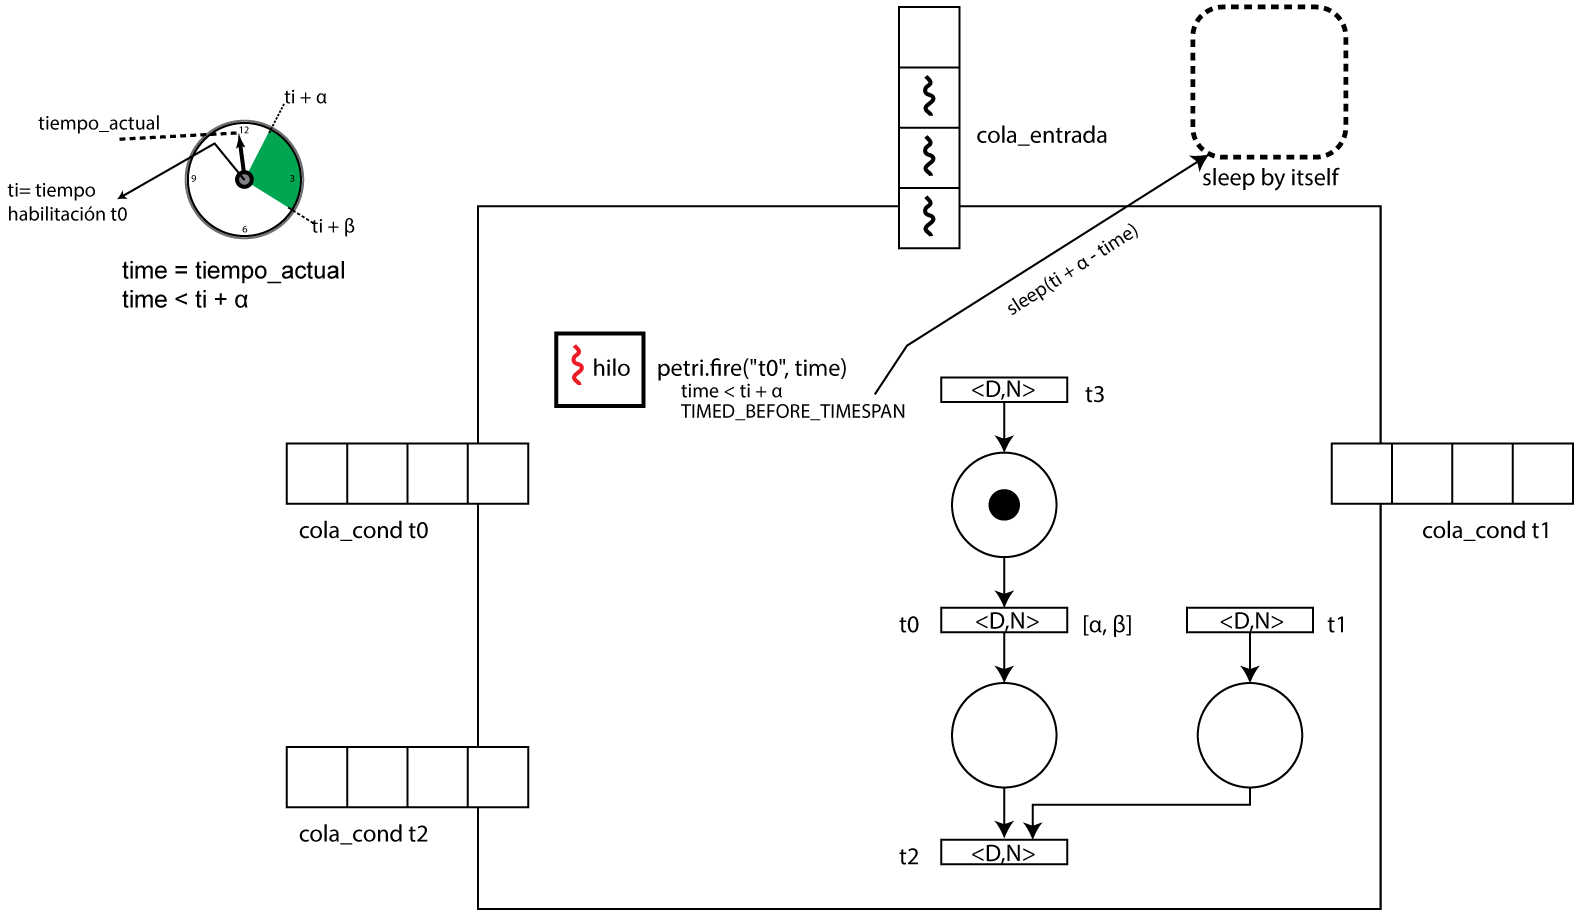
\includegraphics[width=\textwidth]{InversionPrioridad/Inversion_Prioridad_03}}
    \subfigure[El hilo $th_{0}$ libera la entrada y otro hilo ingresa al monitor]
    {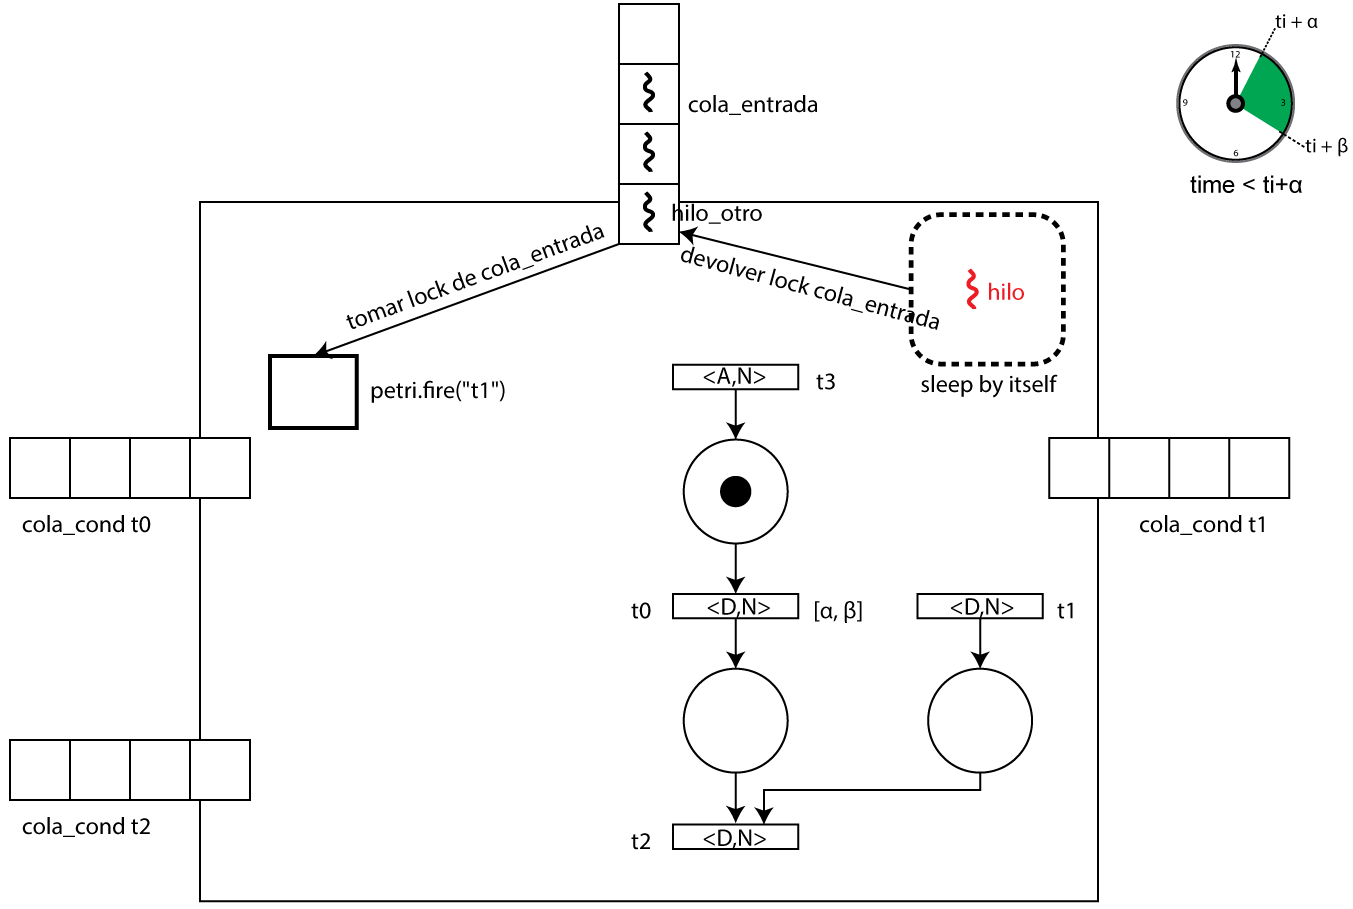
\includegraphics[width=\textwidth]{InversionPrioridad/Inversion_Prioridad_04}}
    \label{fig:Inv_prior_entrada}
\end{figure}
\clearpage
\begin{figure}[H]
    \ContinuedFloat
    \subfigure[El hilo $th_{0}$ va al final de la cola de entrada]
    {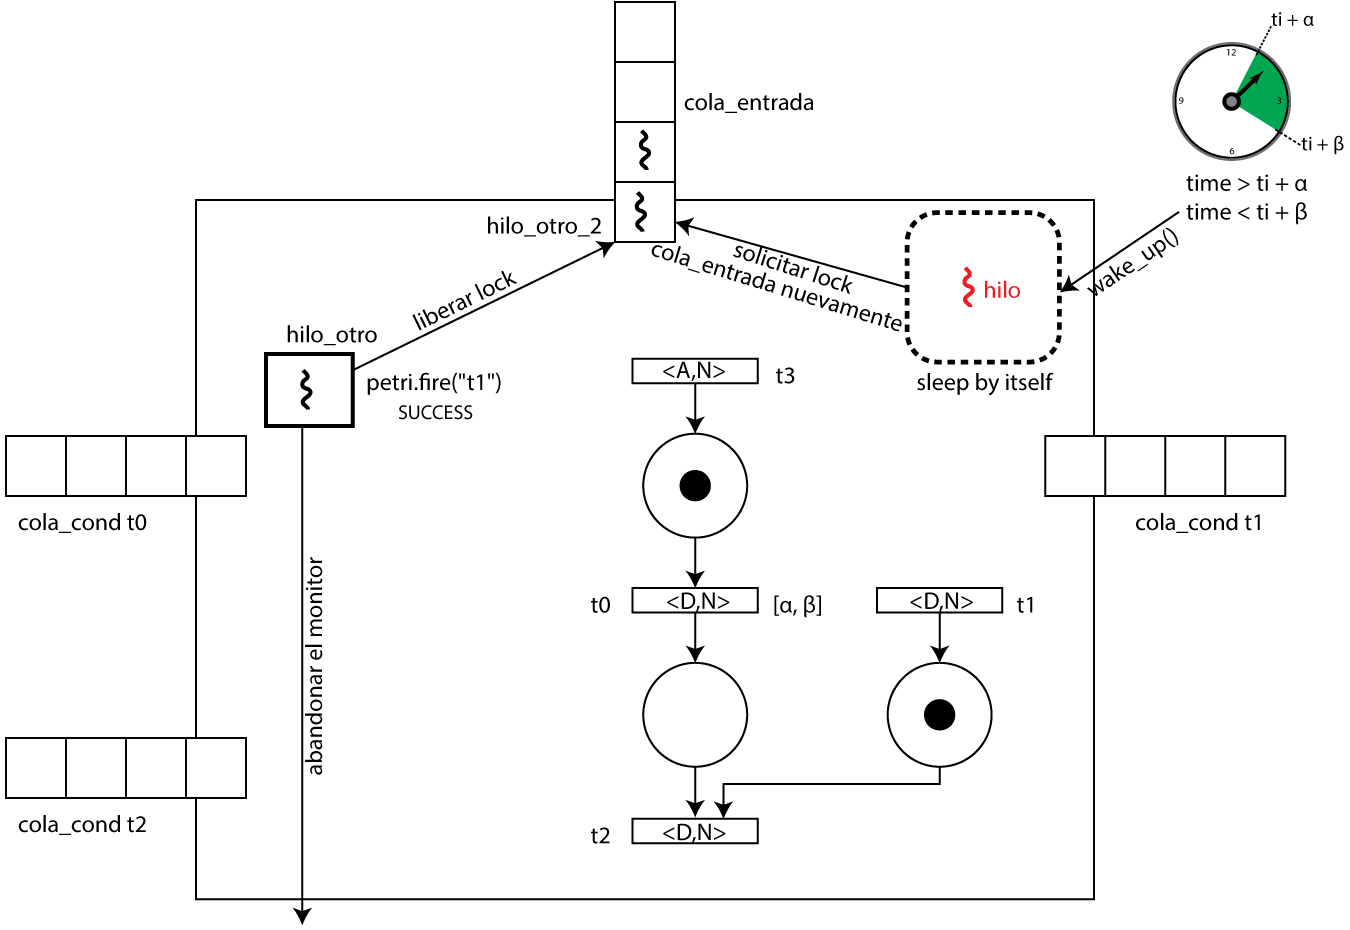
\includegraphics[width=\textwidth]{InversionPrioridad/Inversion_Prioridad_05}}
    \subfigure[Otro hilo se ejecuta]
    {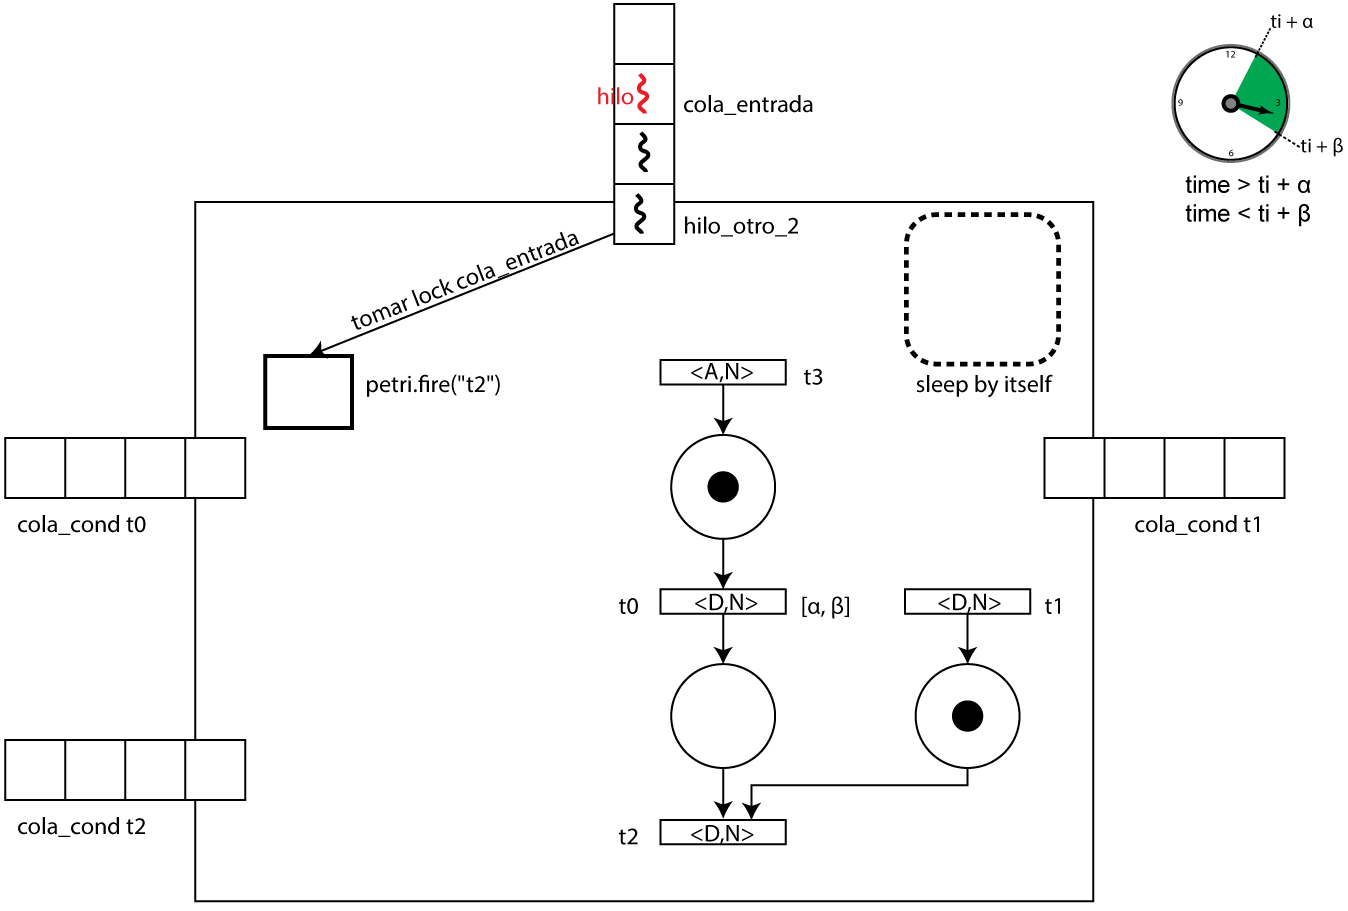
\includegraphics[width=\textwidth]{InversionPrioridad/Inversion_Prioridad_06}}
    \label{fig:Inv_prior_entrada}
\end{figure}
\clearpage
\begin{figure}[H]
    \ContinuedFloat
    \subfigure[Terminó el intervalo de disparo de $t_{0}$ sin que $th_{0}$ logre
    tomar el lock de entrada del monitor]
    {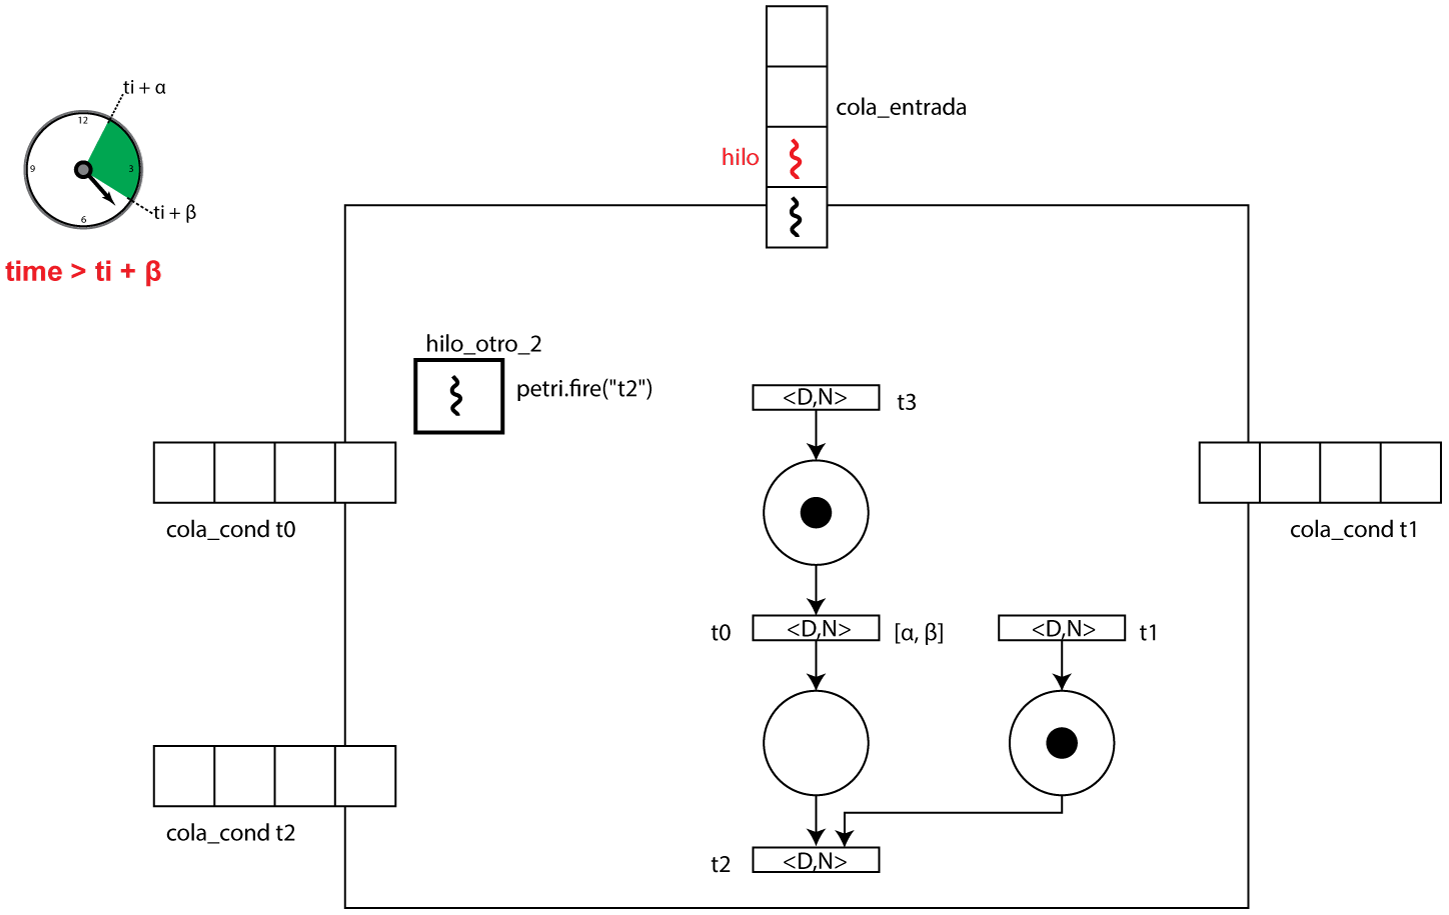
\includegraphics[width=\textwidth]{InversionPrioridad/Inversion_Prioridad_07}}
    \caption{Inversión de prioridades en la cola de entrada del monitor}
    \label{fig:Inv_prior_entrada}
\end{figure}

\subsubsection{Inversión de prioridades en una cola de condición}

Para que se genere una inversión de prioridades en la cola de condición de una
transición, se tienen que dar los siguientes eventos en orden:
\begin{itemize}
  \item Se sensibiliza la transición temporal $t_{0}$ con intervalo $[a,b]$ en
  el instante $t_{i}$
  \item El hilo $th_{0}$ intenta disparar $t_{0}$ en $td < (t_{i} + a)$
  \item El hilo $th_{0}$ libera la entrada y se bloquea temporalmente
  \item Llegan $N$ hilos que intentan disparar a $t_{0}$ y se encolan en su cola
  de condición
  \item El hilo $th_{1}$ toma el lock de entrada y dispara la transición
  $t_{1}$, que deshabilita a $t_{0}$
  \item Cuando $th_{0}$ se desbloquea, toma el lock de entrada e intenta
  disparar $t_{0}$. Como ésta no está sensibilizada, $th_{0}$ va a la cola de
  condición de $t_{0}$
\end{itemize}
 
En este caso, $th_{0}$ se va al final de la cola de condición, cediéndole
incorrectamente su prioridad a los $N$ hilos que llegaron después que él al
monitor a disparar a $t_{0}$.

\subsection{Solución a las inversiones de prioridad}
\label{JPCM_solucion_inv_prioridad}

Analizando los casos de inversión de prioridades expuestos en la sección
anterior, se ve que en ambas oportunidades el problema solucionar modificando
la política de las colas (de entrada y de condición) para gestionar el orden de
dessbloqueo de los hilos por prioridad. De esta manera, un hilo que ya haya
esperado temporalmente puede esperar con prioridad máxima para evitar la
inversión de prioridades.

La forma en que JPCM implementa las colas de prioridad es a través de la clase
\textit{PriorityBinaryLock} (ver figura \ref{fig:JPCM_PetriMonitor_Structure}).
\textit{PriorityBinaryLock} es un lock que implementa dos métodos básicos para
su uso:
\begin{itemize}
  \item \mint{java}|lock(LockPriority priority)|: Su parámetro es opcional y por
  defecto es de baja prioridad. Permite a un hilo tomar el lock. En caso de ya
  estar tomado, el hilo se bloquea en una cola interna.
  \item \mint{java}|unlock()|: Libera el lock. Si existe al menos un hilo en la
  cola despierta al primero.
\end{itemize}

Internamente, \textit{PriorityBinaryLock} utiliza una cola de prioridades para
gestionar los hilos bloqueados que almacena. De esta forma, siendo $A$ y $B$
dos hilos bloqueados en la cola de \textit{PriorityBinaryLock}, $A$ estará más
próximo a ser desbloqueado si:
\begin{itemize}
  \item $A$ tiene mayor prioridad que $B$
  \item $A$ y $B$ tienen la misma prioridad pero $A$ llegó en un instante
  anterior a $B$
\end{itemize}

De esta manera, dentro de un mismo rango de prioridades se respeta el esquema
FIFO utilizado comúnmente en una cola. Y además, se extienden las capacidades
para permitir que un hilo que debe ser atendido con urgencia sea candidato a
salir de la cola antes que uno de menor urgencia.

Al retirar un hilo de la cola, siempre se toma el primero. Es el ordenamiento
el que hace que se respete la gestión de prioridades.

En la siguiente figura se observa la solución al caso de inversión de
prioridades de la sección \ref{inversion_prioridad_cola_entrada}

\begin{figure}[H]
  \centering
    \subfigure[El hilo $th_{0}$ ingresa al monitor]
    {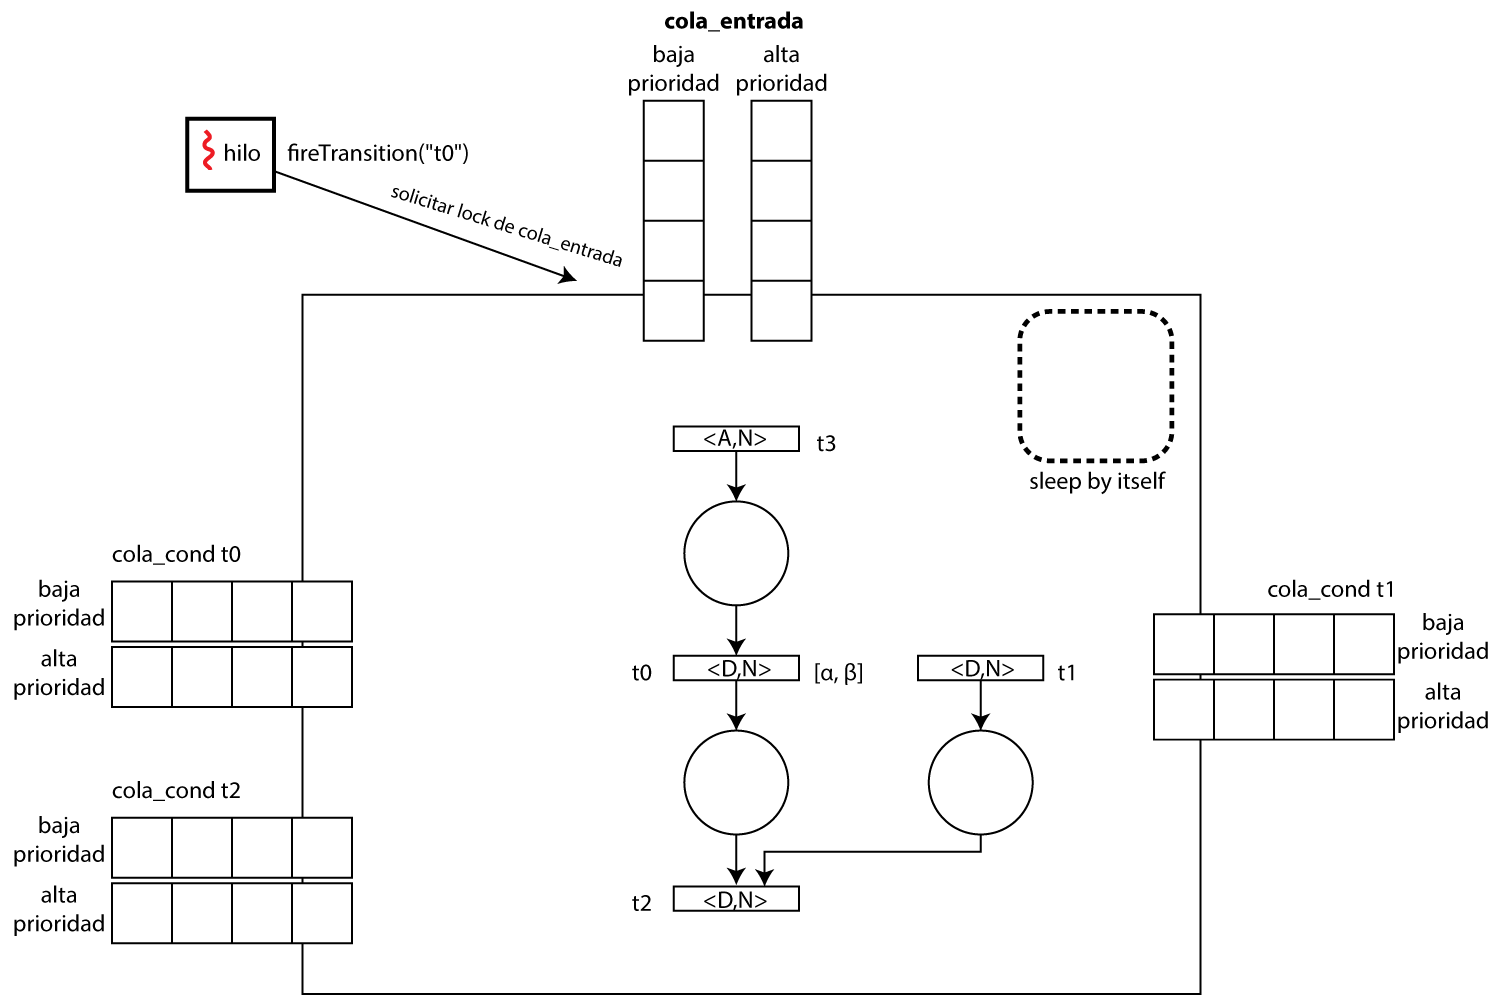
\includegraphics[width=\textwidth]{InversionPrioridad/solucion/Solucion_Inversion_Prioridad_01}}
    \subfigure[Otros hilos intentan tomar el lock del monitor después que $th_{0}$]
    {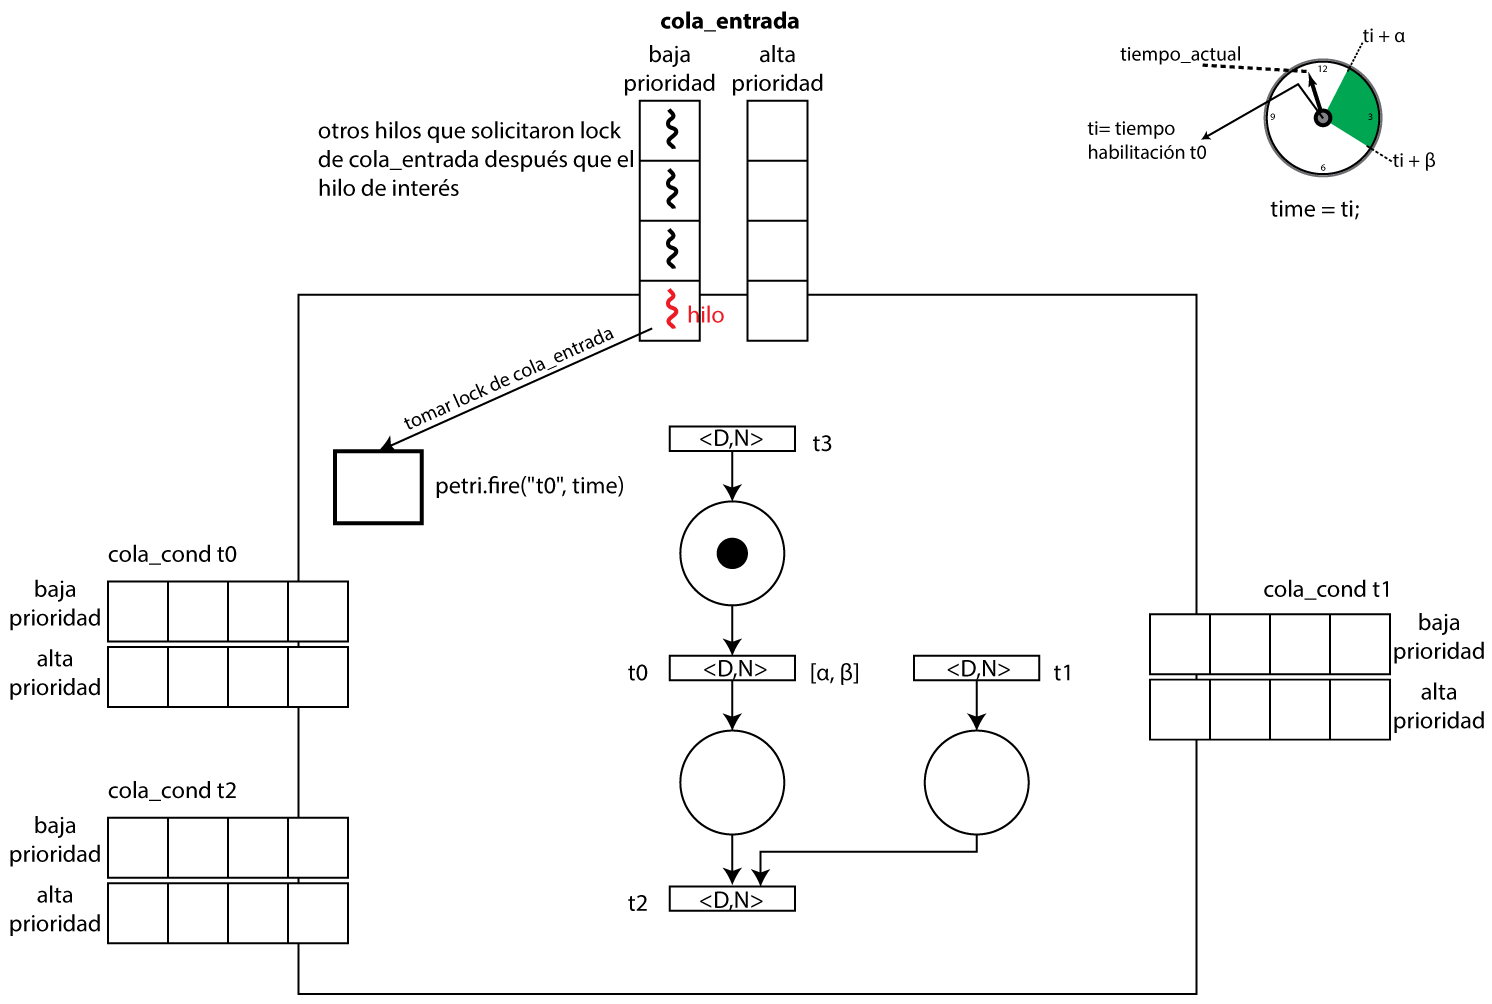
\includegraphics[width=\textwidth]{InversionPrioridad/solucion/Solucion_Inversion_Prioridad_02}}
    \label{fig:Inv_prior_entrada}
    \phantomcaption
\end{figure}
\clearpage
\begin{figure}[H]
    \ContinuedFloat
    \subfigure[El hilo $th_{0}$ intenta disparar $t_{0}$ en $t_{d} < (t_{i} + a)$
    y se bloquea temporalmente ]
    {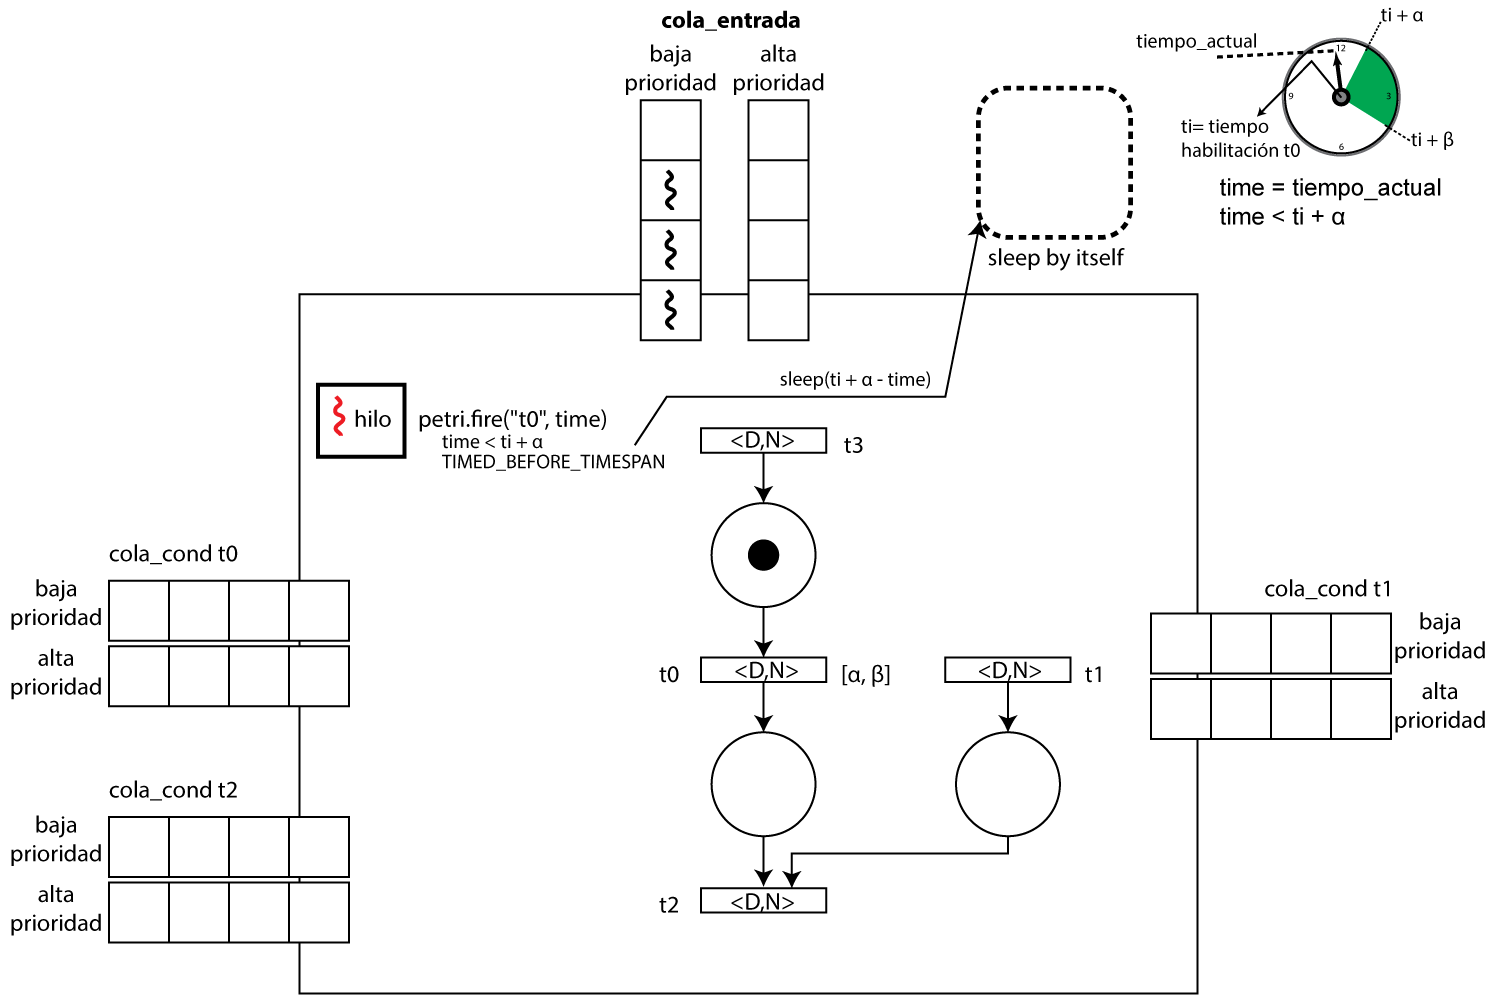
\includegraphics[width=\textwidth]{InversionPrioridad/solucion/Solucion_Inversion_Prioridad_03}}
    \subfigure[El hilo $th_{0}$ libera la entrada y otro hilo ingresa al monitor]
    {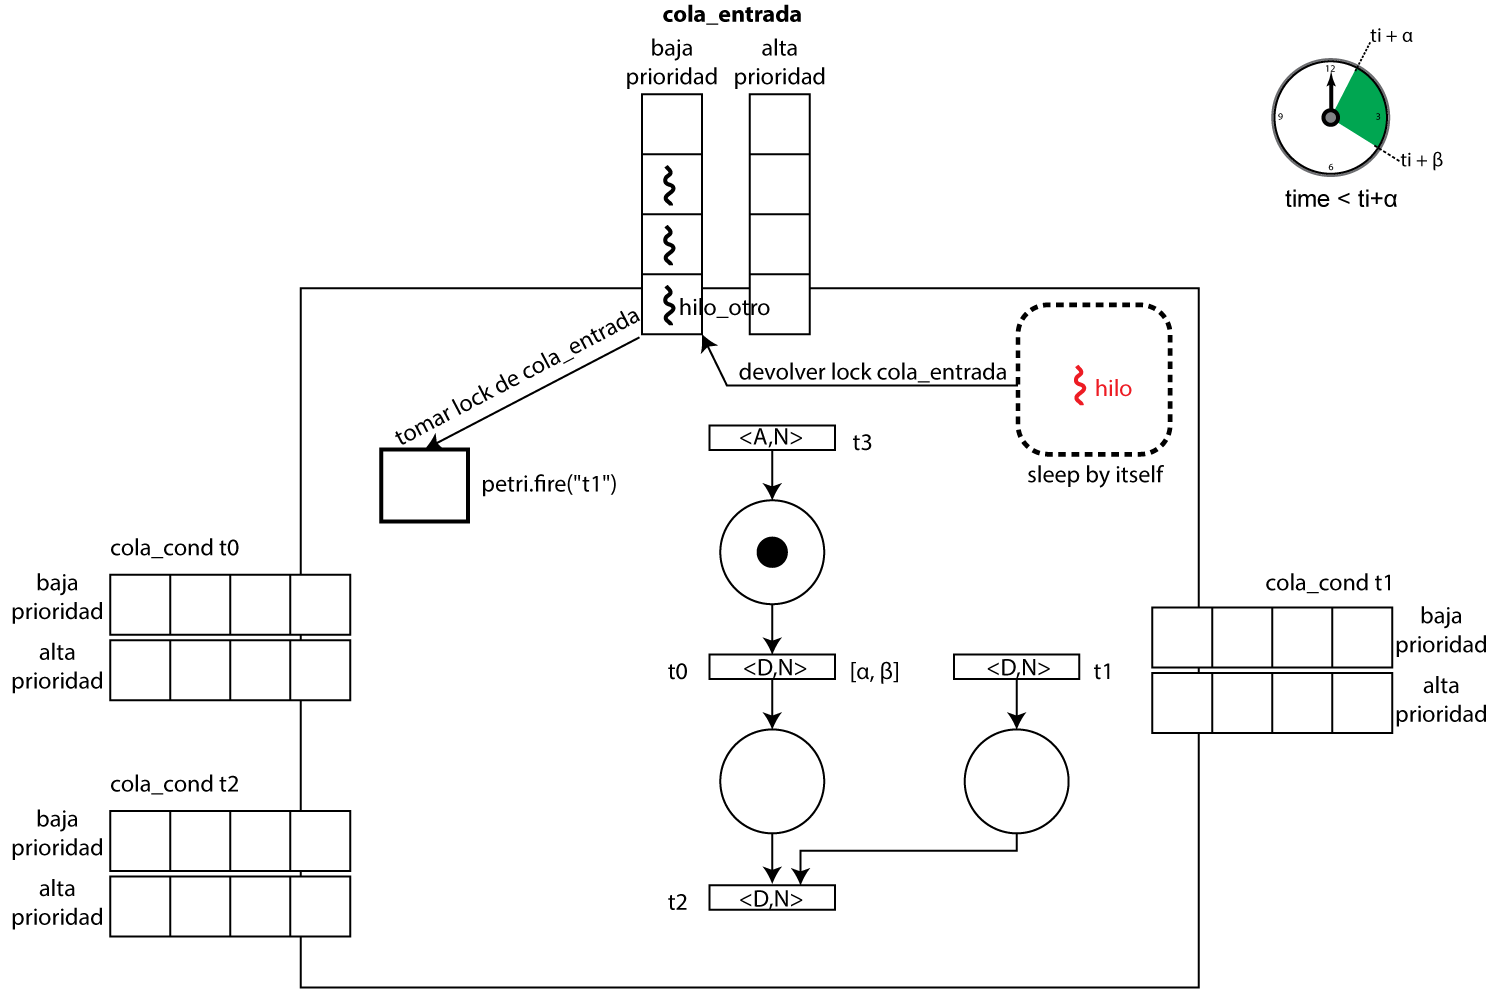
\includegraphics[width=\textwidth]{InversionPrioridad/solucion/Solucion_Inversion_Prioridad_04}}
    \label{fig:Inv_prior_entrada}
\end{figure}
\clearpage
\begin{figure}[H]
    \ContinuedFloat
    \subfigure[El hilo $th_{0}$ va a la cola de entrada con alta prioridad]
    {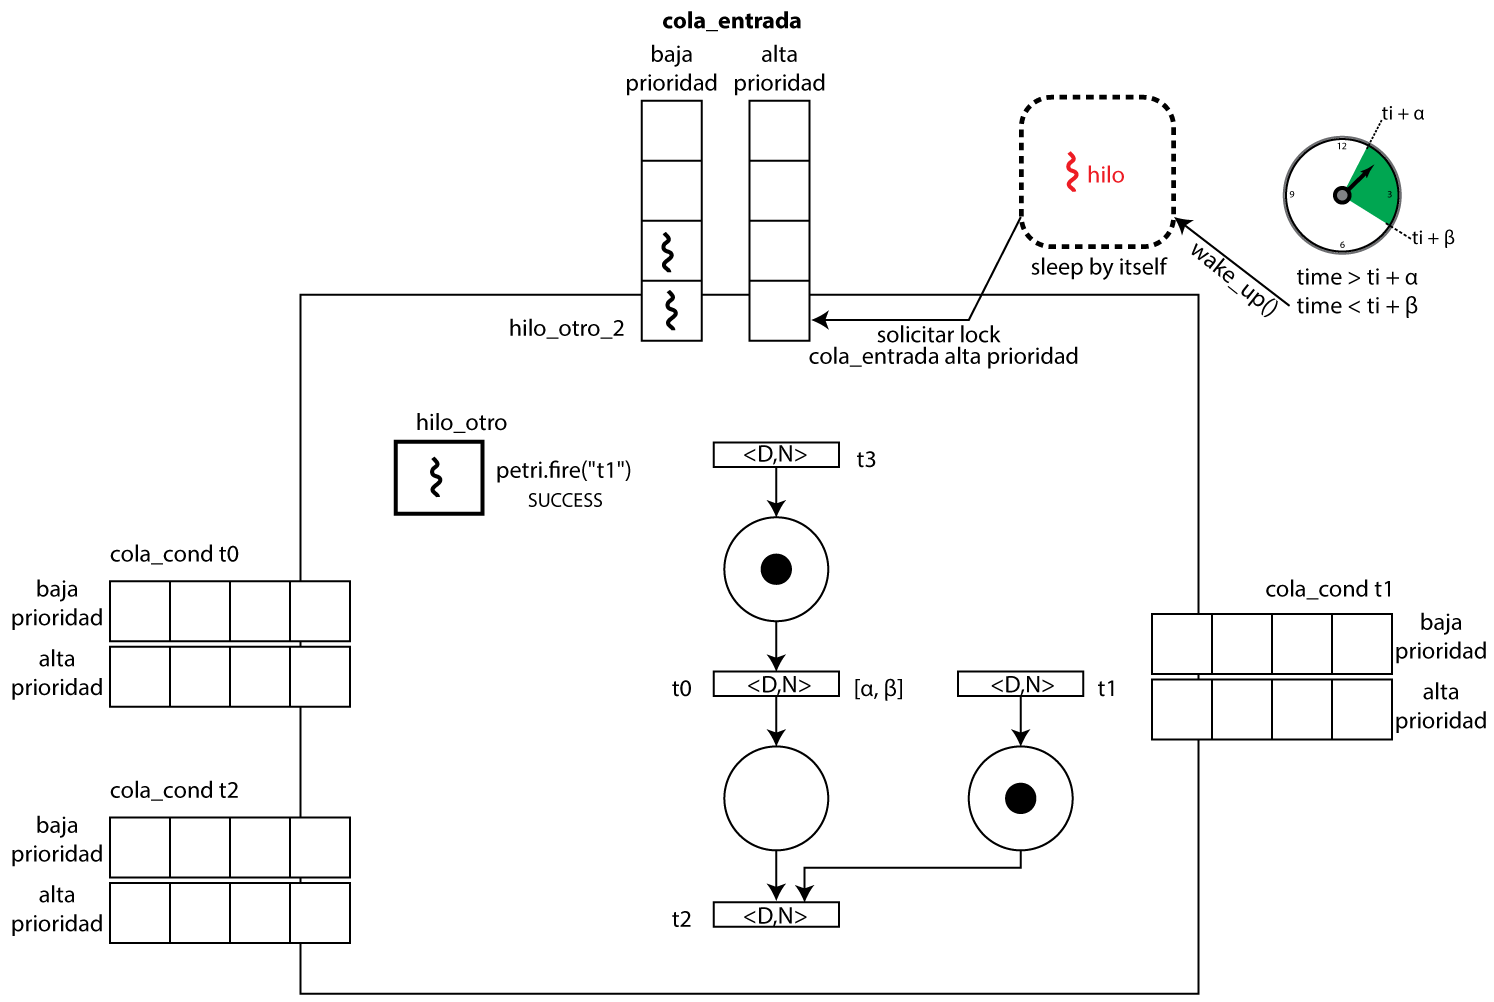
\includegraphics[width=\textwidth]{InversionPrioridad/solucion/Solucion_Inversion_Prioridad_05}}
    \subfigure[Otro hilo se ejecuta y cuando finaliza libera a $th_{0}$ por
    tener la máxima prioridad]
    {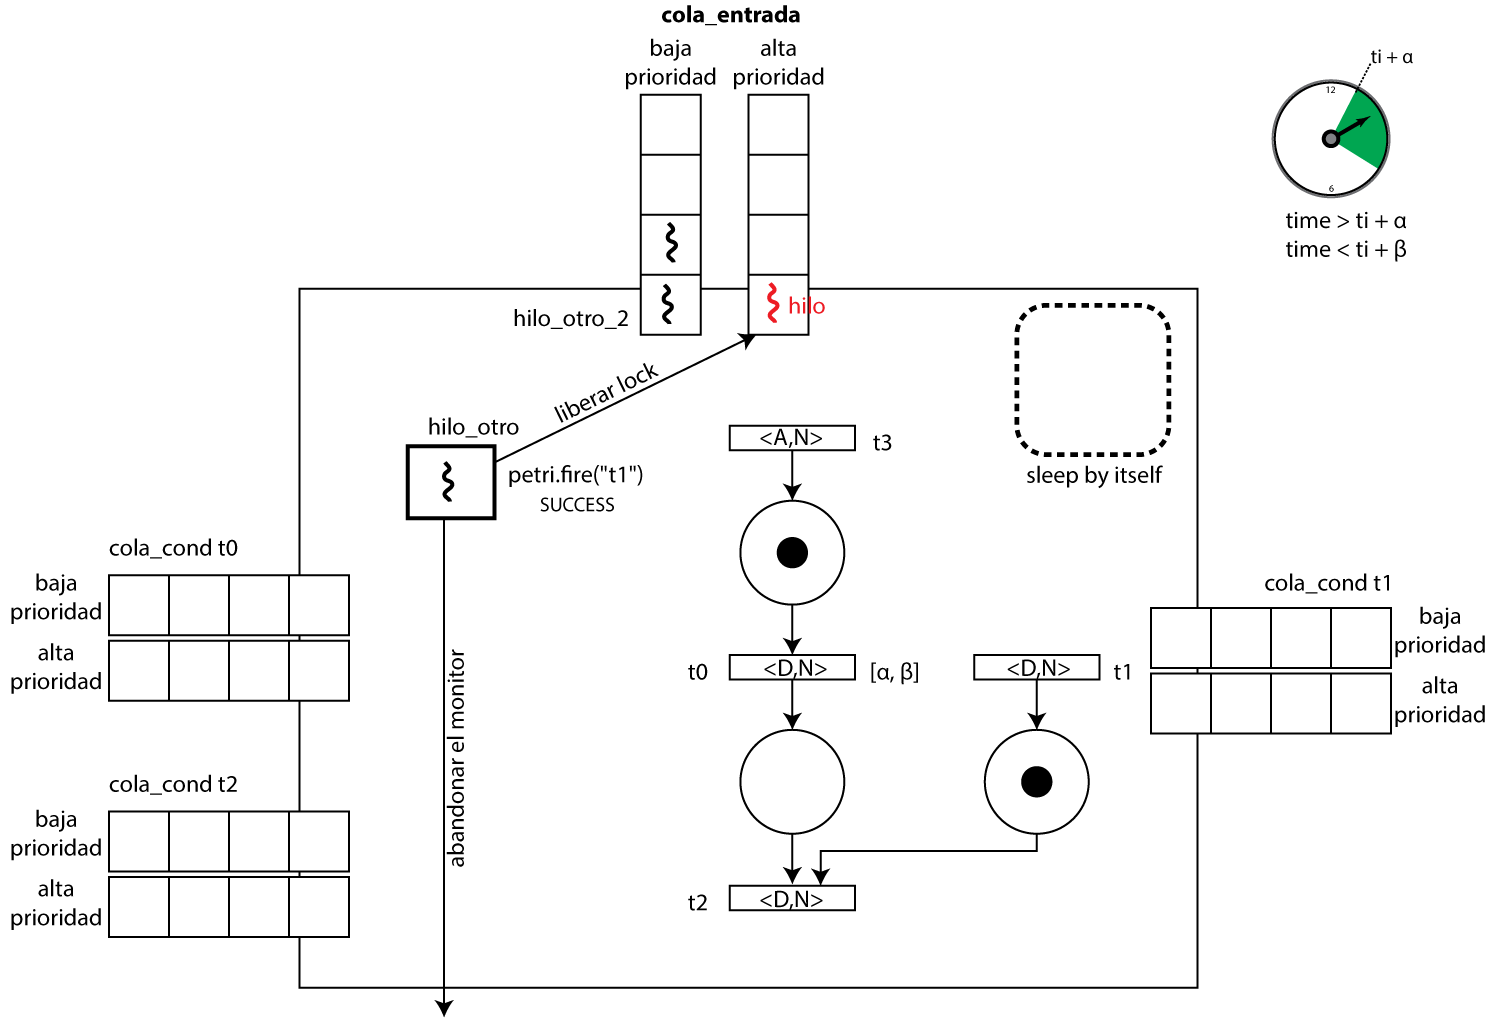
\includegraphics[width=\textwidth]{InversionPrioridad/solucion/Solucion_Inversion_Prioridad_06}}
    \label{fig:Inv_prior_entrada}
\end{figure}
\clearpage
\begin{figure}[H]
    \ContinuedFloat
    \subfigure[$th_{0}$ se desbloquea e intenta disparar $t_{0}$]
    {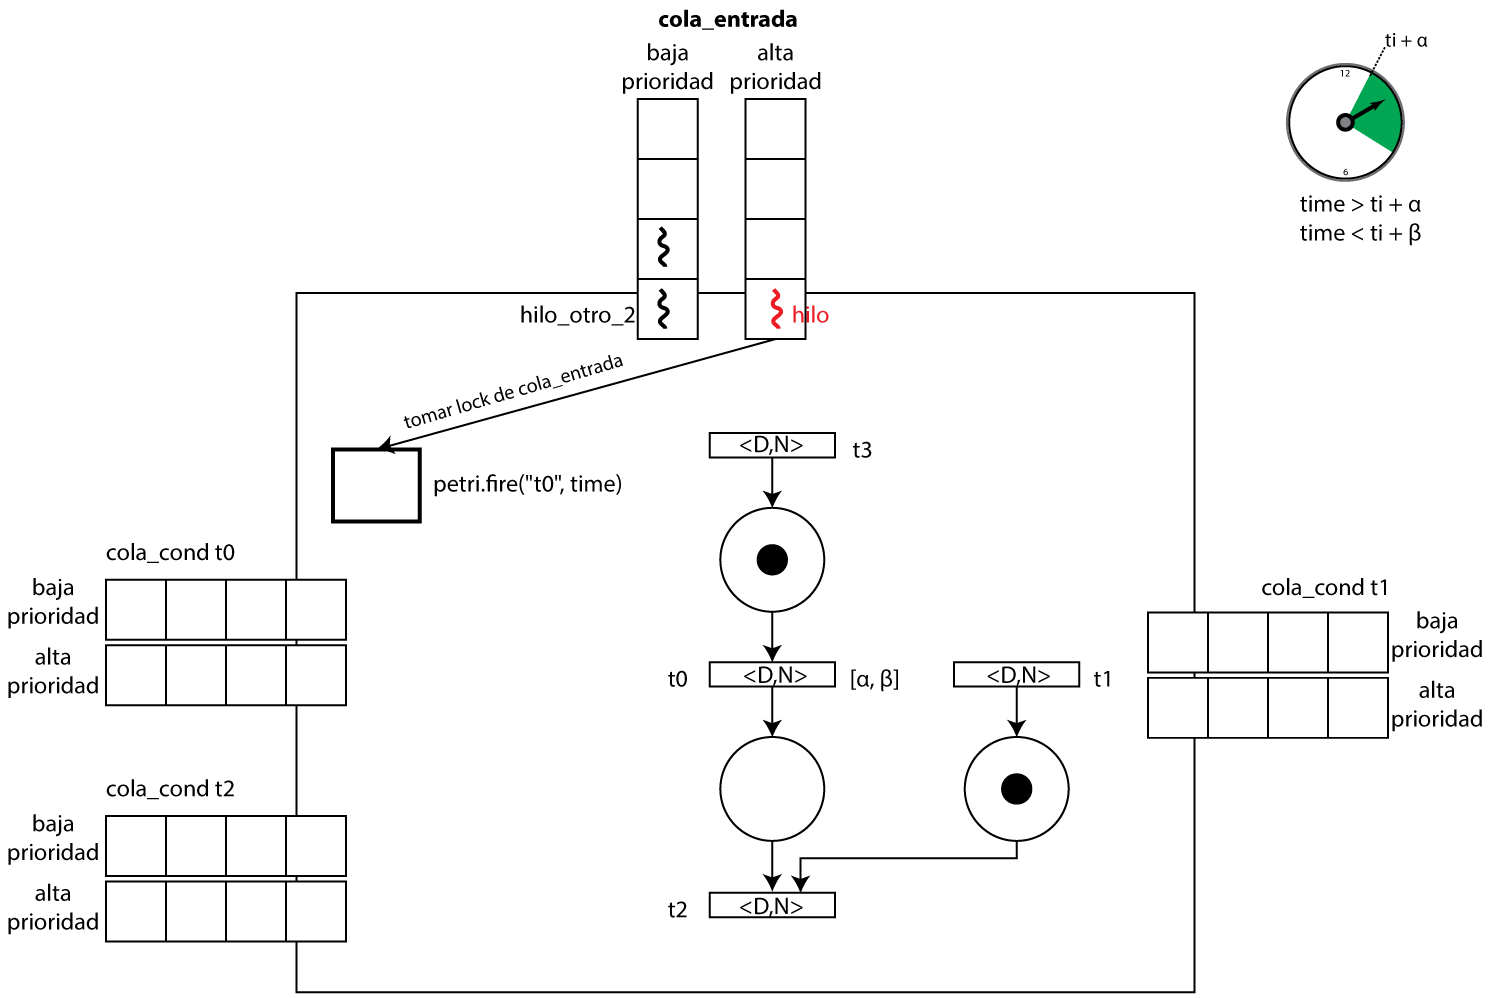
\includegraphics[width=\textwidth]{InversionPrioridad/solucion/Solucion_Inversion_Prioridad_07}}
    \subfigure[$th_{0}$ termina su ejecución y libera el lock de entrada]
    {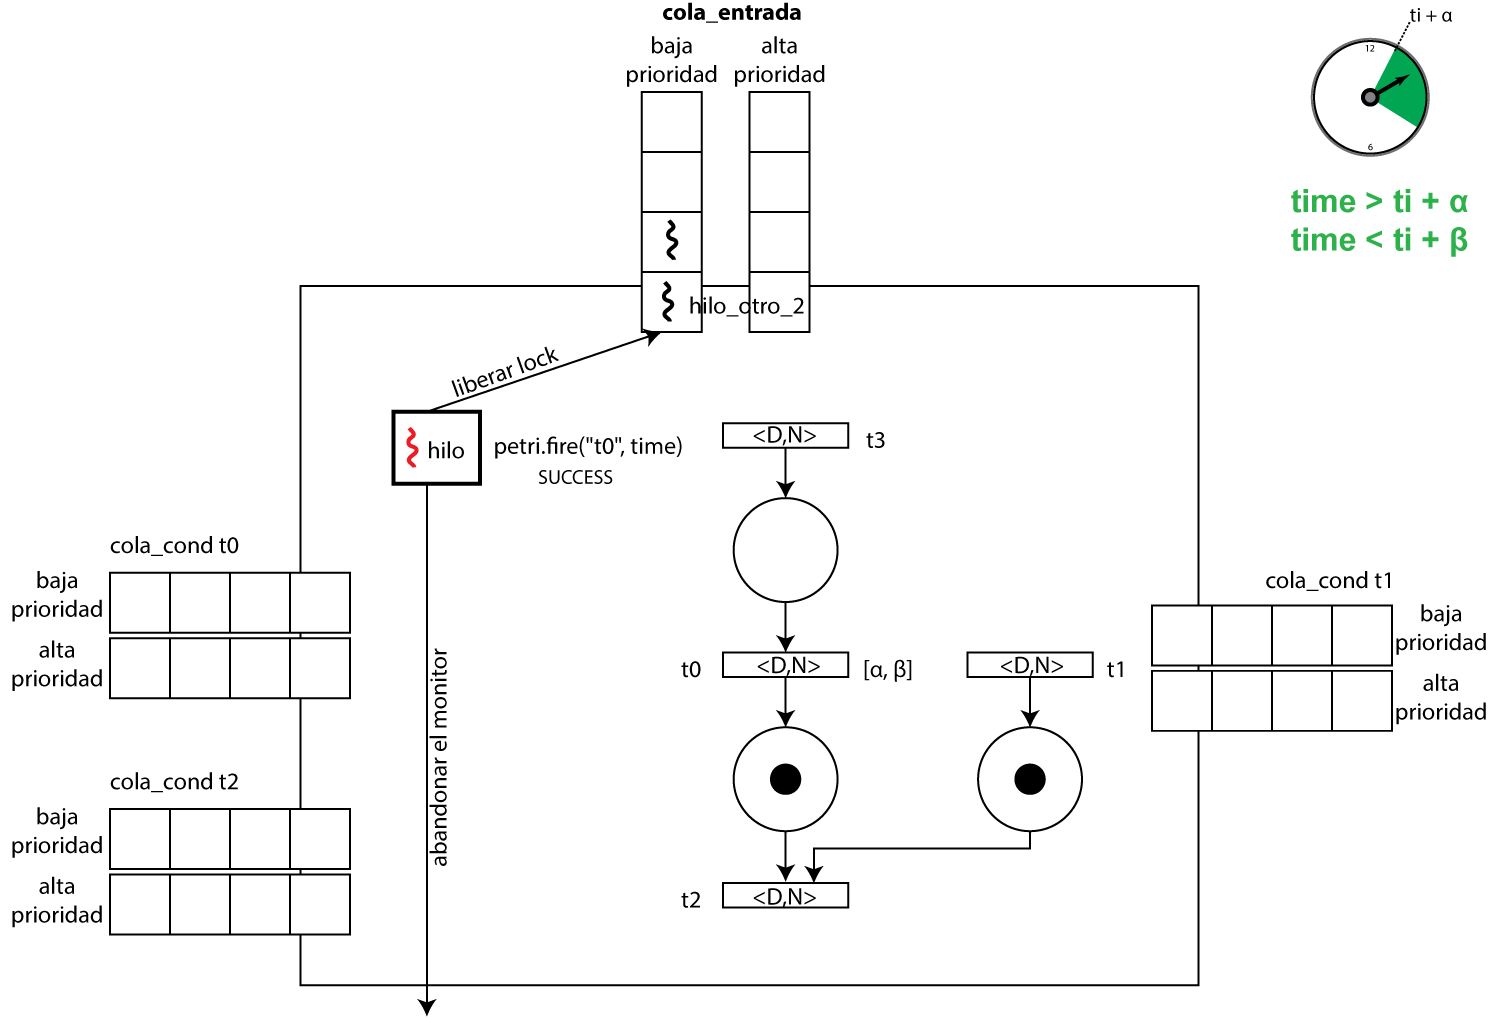
\includegraphics[width=\textwidth]{InversionPrioridad/solucion/Solucion_Inversion_Prioridad_08}}
    \caption{Inversión de prioridades en la cola de entrada del monitor}
    \label{fig:Inv_prior_entrada}
\end{figure}

\subsection{Informes de Disparo de una Transición}

Existen casos en los que es de interés del programador de un sistema que
utilice a JPCM recibir una notificación cuando se produce el disparo de una
transición. Para esto se utilizan las transiciones \textit{informadas} y los
\textit{informes de disparo} (ver sección \ref{informes_disparo}).

Como se puede observar en la figura \ref{fig:JPCM_Fire_SUCCESS}, luego de un
disparo exitoso se envía un evento de disparo. Para que un observador reciba
efectivamente este evento debe haberse suscrito previamente a los eventos de
la transición en cuestión. La suscripción se realiza con la llamada al método
\mint{java}|PetriMonitor.subscribeToTransition()|.

Un intento de suscripción a una transición no informada resulta en el
lanzamiento de una excepción de tipo \mint{java}|IllegalArgumentException| con
un mensaje que explica la situación.

\subsection{Guardas}

Como se explicó en la sección \ref{guardas}, a una transición se pueden asociar
valores booleanos que modifican su semántica de sensibilización. JPCM provee
soporte para guardas con habilitación por valor \mint{java}|true| o por valor
\mint{java}|false|.

Las guardas son cargadas en tiempo de inicialización durante la construcción
del objeto \textit{PetriNet} y son inicializadas con valor \mint{java}|false|.

En cualquier momento un hilo puede modificar el valor de una guarda accediendo
al método \mint{java}|PetriMonitor.setGuard()| con el nombre de la guarda a
modificar y su nuevo valor. Esto está coordinado por el lock de entrada de forma
conjunta con el disparo de una transición para evitar problemas de acceso
concurrente sobre la RdP. Se contempla la posible sensibilización de
transiciones automáticas (donde el hilo que hizo el cambio de valor de la guarda
realiza el disparo) y de transiciones disparadas (en cuyo caso desbloquea a un
hilo que estuviera esperando en su cola de condición si lo hubiera) de la misma
forma que en el disparo de una transición.

Al momento del disparo de una transición, el valor de la guarda asociada
influye en la sensibilización de la misma.
